\documentclass{templufla}          % classe base para a monografia

%==============================================================================
% Utilizacao de pacotes
\usepackage[T1]{fontenc}         % usa fontes postscript com acentos
\usepackage[brazil]{babel}       % hifenização e títulos em português do Brasil
\usepackage[utf8]{inputenc}     % permite edição direta com acentos
\usepackage{amsmath}             % pacote da AMS para Matemática Avançada
\usepackage{amssymb}             % símbolos extras da AMS
\usepackage{latexsym}            % símbolos extras do LaTeX
\usepackage{graphicx}            % para inserção de gráficos
\usepackage{listings}            % para inserção de código
\usepackage{fancyvrb}            % para inserção de saídas de comandos
%\usepackage{enumerate}           % para personalizar lista enumeradas 
											%(incluso na classe)
\usepackage{longtable}           % para tambelas muito grandes NOVO!!!!

\usepackage{colortbl} % cores em tabelas
\newcolumntype{Z}{|>{\columncolor[gray]{0.9}}l|} %cor cinza em células
%\usepackage{array} % já incluso na classe
\newcolumntype{L}[1]{>{\raggedright\let\newline\\\arraybackslash\hspace{0pt}}m{#1}}
\newcolumntype{C}[1]{>{\centering\let\newline\\\arraybackslash\hspace{0pt}}m{#1}}
\newcolumntype{R}[1]{>{\raggedleft\let\newline\\\arraybackslash\hspace{0pt}}m{#1}}
\usepackage{multirow} % para juntar duas linhas em uma só

\usepackage{multicol} % para uso de várias colunas

% cores para os links cruzados
\usepackage{xcolor}
\definecolor{rltred}{rgb}{0.2,0,0}
\definecolor{rltgreen}{rgb}{0,0.2,0}
\definecolor{rltblue}{rgb}{0,0,0.2}

\usepackage[colorlinks=true,
            urlcolor=rltblue,       % \href{...}{...} external (URL)
            filecolor=rltgreen,     % \href{...} local file
            linkcolor=rltred,       % \ref{...} and \pageref{...}
            citecolor=rltgreen,
            pdftitle={Template de Trabalhos acadêmcios UFLA},
          pdfauthor={João Autor},
          pdfsubject={Template de Trabalhos acadêmcios UFLA.},
          pdfkeywords={Comunicação Científica. 2. Pesquisa . 3. Pesquisa Científica. 
 					 4. Redação. 5. Monografia.}%
]{hyperref} % para referência cruzadas
%\usepackage{hyperref}            % para referência cruzadas
\usepackage{subfigure}           % figuras dentro de figuras
\usepackage{caption}            % remodelando o formato dos títulos de 
                                 % tabelas e figuras

% configuração padrão do listings   
\lstset{
   language=Java,
   extendedchars=true,
   tabsize=3,
   basicstyle=\footnotesize\ttfamily,
   stringstyle=\em,
   showstringspaces=false ,
   inputencoding=utf8,
   literate={á}{{\'a}}1 {é}{{\'e}}1 {í}{{\'i}}1 {ó}{{\'o}}1 {ú}{{\'u}}1
   			{Á}{{\'A}}1 {É}{{\'E}}1 {Í}{{\'I}}1 {Ó}{{\'O}}1 {Ú}{{\'U}}1
   			{â}{{\^a}}1 {ê}{{\^e}}1 {ô}{{\^o}}1
   			{Â}{{\^A}}1 {Ê}{{\^E}}1 {Ô}{{\^O}}1
            {ã}{{\~a}}1 {õ}{{\~o}}1 {ẽ}{{\~e}}1 
            {ç}{{\c{c}}}1
            {à}{{\`{a}}}1{À}{{\`{A}}}1,
}

% para referências de acordo com a ABNT
% precisa instalar o abntex2 antes!!!
% http://abntex.codigolivre.org.br/
% comente se pretende usar outro padrão

%abnt-emphasize=bf coloca o título das bibliografias em negrito
%abnt-thesis-year=both
\usepackage[alf, abnt-etal-list=3, abnt-url-package=url, abnt-emphasize=bf]{abntex2cite}


% evite usar o hyperref com abntex, pode dar caca em urls... no linha anterior, informo
% para incluir urls usando o pacote url e não o hyperref
%
% caso queira o hyperref com abntex, comente a linha anterior e descomente a seguinte
%\usepackage[alf,abnt-etal-cite=3,abnt-etal-list=0,abnt-etal-text=emph]{abntex2cite}
%
% caso vc ainda use a versão anterior da abntex, comente a linha incluindo o abntex2cite
% e descomente a próxima linha 
%\usepackage[alf,abnt-etal-cite=3,abnt-etal-list=0,abnt-etal-text=emph]{abntcite}


%==============================================================================
% criação do glossário, listas de siglas, símbolos e etc
\loadglsentries{glossarios/abreviaturas}
\loadglsentries{glossarios/glossario}
\loadglsentries{glossarios/siglas}
\loadglsentries{glossarios/simbolos}
%==============================================================================

%==============================================================================
% para os fãs do Word, descomente as linhas abaixo
%\sloppy %mais espaço entre as linhas
%\usepackage{identfirst} %identando-se a primeira linha de cada seção
%\noindentfirst % Tire o comentário para manter o padrão do LaTeX.

%==============================================================================
% definido comandos na monografia - não é necessário na sua monografia 
% apenas para exemplificar a definição de novos comandos
\newcommand{\defs}[1]{\textsl{#1}}


% Especificando hifenizações que por ventura LaTeX não saiba fazer
% Por padrão 99,9% dos termos em português devem ser hifenizados corretamente.
\hyphenation{hardware software Li-nux am-bien-te diag-nos-ti-car coor-de-na-ção 
FAE-PE Recovery TelEduc Williams UFLA}

%==============================================================================
% Dados da monografia, capa: autor, titulo, banca, etc... - SUBSTITUA DE ACORDO
%==============================================================================
\author{Joana Autora da Silva}
\title{Template de Exemplo do Estilo Padrão UFLA}
\subtitle{Usando Latex! =)}
\engtitle{Example Template for UFLAS' Standard Style}
\engsubtitle{Using \LaTeX =)}
\edicao{6$^a$ edição atualizada, ampliada e revista}
\date{2025}
\tipo{Tese apresentada à Universidade Federal de Lavras, como parte das exigências do Programa de Pós-Graduação em Monografia, área de concentração em TCC, para a obtenção do título de Doutor.}
% use \orientador ou \orientadora quando for o caso
\orientador{Prof. DSc. José Orientador}
%\orientadora{}
% use \coorientador ou \coorientadora quando for o caso
\coorientadora{Prof. DSc. Maria Orientadora } % comente se não tiver coorientador
%\coorientador{}
\local{Lavras -- MG}
\bancaum{Prof. MSc. Antônio Banca Um}{UFM}
\bancadois{Prof. DSc. João Banca Dois}{FCO} % comente se sua banca tiver só um professor
\bancatres{Profa. Esp. Eliza Banca Três}{BELMIS}
\bancaquatro{Prof. Esp. Zorbison Uberplax IV}{UFO}
\defesa{11 de abril de 2025}
%==============================================================================
%##################################################
% Dados para Ficha catalográfica, gerada pelo sistema da Biblioteca da UFLA
% http://www.biblioteca.ufla.br/FichaCatalografica/
% dados para ficha catalográfica
% Elaboração da Ficha Catalográfica
\preparofichacat{Ficha catalográfica elaborada pela Coordenadoria de Processos Técnicos da Biblioteca Universitária da UFLA, com dados informados pelo(a) próprio(a) autor(a).}
% primeiro autor - como na primeira linha da ficha catalográfica
\fcautor{Silva, Joana Autora da}
% autores, separados por vírgula - na ficha catalográfica, no formato que
% vem após o título e a barra ("/")
\fcautores{Joana Autora da Silva, João Autor do Silvo}
% Numero de páginas, caso o valor seja diferente do calculado, 
% basta descomentar e adicionar.
%\fcnpaginas{777}
% caso trabalho seja ilustrado (figuras, gráficos, tabelas, etc.), 
% então informar por meio do comando a seguir
% caso não seja ilustrado, basta comentá-lo
\fcilustrado{il.}
% dados da edição para a ficha 
\fcedicao{6$^a$ ed. rev., atual. e ampl.}
% tipo do trabalho (tese, dissertação, etc.), de acordo com sistema
% de geração de ficha catalográfica
\fctipo{Tese(doutorado)}
% ano da defesa, só precisa informar se for diferente do ano da publicação
% se forem iguais, comente a linha a seguir
\fcdatadefesa{2025}
% preencher aqui com os dados de catalogação gerados pelo sistema
\fccatalogacao{1. TCC. 2. Monografia. 3. Dissertação. 4. Tese. 5. Trabalho Científico – Normas. I. Universidade Federal de Lavras. II. Título.}
\fcclasi{808.066}

%##################################################

%\antesfichacat{\noindent Para citar este documento: \\UNIVERSIDADE FEDERAL DE LAVRAS. Biblioteca Universitária. \textbf{Manual de normalização e estrutura de trabalhos acadêmicos: TCC, monografias, dissertações e teses}. 2. ed. rev., atual. e ampl. Lavras, 2015. Disponível em: \url{http://www.biblioteca.ufla.br/wordpress/wpcontent/uploads/bdtd/manual_normalizacao_UFLA.pdf}. Acesso em: data de acesso.}

%\depoisfichacat{\noindent A reprodução e a divulgação total ou parcial deste trabalho são autorizadas, por qualquer meio convencional ou eletrônico, para fins de estudo e pesquisa, desde que citada a fonte.\\
%\newline
%{\small Este documento possui páginas em branco para facilitar a impressão frente-e-verso.}}

%##################################################

%##################################################

% para os exemplos do manual
%\newenvironment{exemplomanual}{
%\vspace{0.5cm}
%\noindent\begin{minipage}{\textwidth}
%\noindent\rule{\textwidth}{0.5pt}
%\vspace{-1cm}
%\begin{flushleft}
%}{
%\end{flushleft}
%\vspace{-0.6cm}
%\noindent\rule{\textwidth}{0.5pt}
%\vspace{0.3cm}
%\end{minipage}
%}

%\newenvironment{exemplomanuallista}{
%\vspace{0.3cm}
%\noindent\begin{minipage}{\textwidth - 0.5cm}
%\noindent\rule{\textwidth}{0.5pt}
%\vspace{-1cm}
%\begin{flushleft}
%}{
%\end{flushleft}
%\vspace{-0.6cm}
%\noindent\rule{\textwidth}{0.5pt}
%\vspace{0.3cm}
%\end{minipage}
%}

% por conta de alguns exemplos
%\usepackage{setspace}

%##################################################

% se vc já defendeu e tem o arquivo escaneado da folha de rosto, 
% descomente e altere o nome do arquivo
%\folhaAprovacaoAssinada{folharosto}

% Aqui começa o documento propriamente dito
\begin{document}

\maketitle

\dedic{Espaço reservado à dedicatória.}     % Dedicatórias\\

\thanks{Espaço reservado aos agradecimentos.}         % Agradecimentos

\epigrafe{ % citação opcional
Espaço reservado à epígrafe.\\
(Autor Desconhecido)}


% palavras-chave
\palchaves{Resumo; Palavras; Representativas.}
\resumo{Mudanças com relação ao original (Uflamon 3a Edição):\\
> Alteração para fonte do texto 12pt, folha a4 e onesided;\\
> Alteração no tamanho das margens;\\
> Adição dos indicadores de impacto;\\
> Coorientador(a) agora aparece na ficha catalográfica;\\
> Nome da/do autor(a) mais alto na capa;\\ 
> Adição de glossários, listas de termos e índices;\\
> Remoção de páginas duplas dos elementos pré-textuais;\\
> Remoção de <> entre links na referências;\\
> Reorganização dos arquivos;\\
> Uso de itálico nas expressões em latim nas referências (ex: \textit{et al} e [\textit{s.n.}]);\\
> Alteração na capitalização de citações de pessoas físicas (de AUTOR para Autor);\\
> Remoção do salto de linha entre o título e subtítulo;\\
> Suporte para mais de 26 anexos/apêndices (abençoado seja quem usar isso);\\
> Agora as listas de figuras e etc mantêm a formatação para qualquer índice (antes, figuras/tabelas > 10 quebravam a formatação);\\
> Agora o sumário mantém a formatação para qualquer índice (antes, sec/subsec > 10 quebravam a formatação);\\
> Logo da UFLA agora é em formato vetorial (resolução "infinita");\\
> Alteração de Large de 14.4pt para 14pt;\\
> Alteração de small de 10.95pt para 11pt;\\
> Uso de 12pt para títulos de figuras e tabelas;\\
> Uso de 11pt para notas, fichas e rodapés;\\
> Ajustes de posicionamento necessário graças às diferenças de tamanho das fontes e das margens;\\
> Adicionado suporte para acentos e ç nos listings;\\
\\
Se encontrar mais mudanças necessárias, por favor informar!\\
Contato:\\
https://github.com/joaopaulo7/Template-Trabalhos-Academicos-UFLA (preferêncial)\\
joao.lima10@estudante.ufla.br\\
}  % Resumo (digite aqui o resumo)

% keywords devem vir antes do abstract
\keywords{Summary; Words; Representative.} % keywords
\abstract{The abstract should contain representative words of the work content, located below the abstract, separated by two spaces, preceded by the keyword expression. These representative words are spelled with the first letter capitalized, separated by point.}


\indicadoresdeimpacto{De caráter institucional, é um item obrigatório como parte das exigências das PRPG/PROEC para os trabalhos de pós-graduação Stricto sensu da UFLA. O autor deve apresentar um relato dos impactos sociais, tecnológicos, econômicos e/ou culturais dos resultados obtidos, considerando as populações, sociedade e territórios, deixando evidente se esses impactos foram concretos e diretos ou em potencial. Ao elaborar o item sobre impactos, é importante: 
a) caracterizar e quantificar resultados dos impactos sociais, tecnológicos, econômicos e/ou culturais da melhor forma possível; 
b) estabelecer se há algum caráter extensionista no trabalho, demonstrando impacto e participação da sociedade externa à UFLA, como parceiros e público-alvo; 
c) definir o território e grupos populacionais impactados; 
d) quando possível, declarar público diretamente beneficiado e número de docentes, estudantes e técnicos envolvidos nas ações extensionistas; 
e) estabelecer em quais das oito áreas temáticas da Política Nacional de Extensão podem ser classificados os impactos do trabalho. São elas: 1 - Comunicação, 2 - Cultura, 3 - Direitos humanos e justiça, 4 - Educação, 5 - Meio ambiente, 6 - Saúde, 7 - Tecnologia e produção e 8 - Trabalho;
 f) demonstrar quais os impactos da pesquisa e se estão alinhados com os 17 (dezessete) Objetivos de Desenvolvimento Sustentável (ODS) da Organização das Nações Unidas (ONU).}

\impactindicators{Of an institutional nature, it is a mandatory item as part of the PRPG/PROEC requirements for UFLA's Stricto sensu postgraduate work. The author must present a report on the social, technological, economic and/or cultural impacts of the results obtained, considering the populations, society and territories, making it clear whether these impacts were concrete and direct or potential. When preparing the item on impacts, it is important to:
a) characterize and quantify the results of the social, technological, economic and/or cultural impacts in the best possible way;
b) establish whether there is any extensionist character to the work, demonstrating the impact and participation of society outside UFLA, such as partners and target audience;
c) define the territory and population groups impacted;
d) when possible, declare the public directly benefited and the number of teachers, students and technicians involved in the extension actions;
e) establish in which of the eight thematic areas of the National Extension Policy the impacts of the work can be classified. They are: 1 - Communication, 2 - Culture, 3 - Human rights and justice, 4 - Education, 5 - Environment, 6 - Health, 7 - Technology and production and 8 - Work;
f) demonstrate the impacts of the research and whether they are aligned with the 17 (seventeen) Sustainable Development Goals (SDGs) of the United Nations (UN).}

%##################################################

% Dados do guia
%\begin{titlepage}
%\pagestyle{empty}
%\renewcommand{\baselinestretch}{1}
%\enlargethispage{1.5cm}
%\input{reitoria}
%\cleardoublepage
%\end{titlepage}

%##################################################

% descomente para habilitar a lista desejada
\listoffigures                             % Lista de Figuras
%\listofilustracoes
%\listofgraficos						   % Lista de Gráficos
\listoftables                              % Lista de Tabelas
\listofquadros							   % Lista de Quadros
%\listofexemplos
%\listofteoremas
\listofabreviaturas
\listofsiglas
\listofsimbolos
\tableofcontents                           % Sumário

\clearpage

\pagestyle{ufla}

%==============================================================================
% incluindo as seções
\chapter{\MakeUppercase{Introdução}}

O objetivo deste documento é apresentar o uso básico da classe \texttt{templufla} para a elaboração de trabalhos acadêmicos da \glsxtrfull{ufla}, utilizando a linguagem de marcação \LaTeX\ \cite[ p.17]{Lamport1994}. A maioria dos comandos (macros) e ambientes das classes básicas da linguagem é válida também nessa classe, que é estendida com comandos para confecção da capa, páginas de rosto, dedicatórias, etc. A classe atual foi baseada na classe \texttt{uflamon}, disponível em CC-BY 4.0, no site Overleaf.

Inicialmente, a classe \texttt{uflamon} foi criada de acordo com as normas da PRPG/UFLA para produção de TCC \cite{PRPG2006}. Essas normas foram posteriormente atualizadas, de maneira geral pela UFLA, para a produção de monografias, dissertações e teses \cite{BIB2010}. A classe \texttt{uflamon} foi mantida até a 2ª edição da normalização da \gls{ufla} \cite{UFLA:2015}.

Então, em 2025, com a publicação da 6ª edição da normalização \cite{UFLA:2025}, os atuais mantenedores criaram a classe \texttt{templufla} e o atual template, adaptando o antigo código para a nova norma, corrigindo inadequações, atualizando pacotes e ampliando o formato.

Este texto, com o objetivo de familiarizar o usuário da linguagem \LaTeX\ e demonstrar o uso da classe \texttt{templufla}, encontra-se organizado da seguinte maneira: 

A \autoref{sec:latex} apresenta conceitos básicos da linguagem \LaTeX, servindo como um ponto de início para novos usuários. 
A \autoref{sec:template} demonstra como utilizar os elementos da classe para a criação de trabalhos no formato da \gls{ufla}.
A \autoref{sec:listasEGlossario} é um tutorial básico de como usar os pacotes \texttt{glossaries} e \texttt{imakeidx} para criar listas, glossário e índice. 
A \autoref{sec:conclusao} apresenta comentários e observações finais.
Por fim, os Anexos \ref{anex:lorem1} e \ref{anex:lorem2} demonstram o uso dos anexos e o \autoref{apen:apendice} mostra como elaborar um apêndice simples.
\chapter{\MakeUppercase{Utilizando a Classe no Formato da UFLA}}\label{sec:template}

Agora que já temos o conhecimento básico sobre como a linguagem \LaTeX\ funciona, podemos nos aprofundar nos detalhes de como utilizar esse template (e, especialmente, a classe \texttt{templufla}) para gerar documentos padronizados de alta qualidade.

\section{Sobre as Seções (seção secundária)}\label{sec2:secoes}
\subsection{Sobre as Seções (seção terciária com texto extra comicamente grande para testar como será a quebra de linha do título)}\label{sec3:teste}
\subsubsection{Sobre as Seções (seção quaternária)}\label{sec4:teste}
\subsubsubsection{Sobre as Seções (seção quinária)}\label{sec5:teste}

Um dos fatores fundamentais no desenvolvimento de um trabalho acadêmico é sua organização. Na normalização da UFLA e da ABNT, os trabalhos podem ter formato de livro, como esse template, mas devem ser divididos em seções, não em capítulos e todo o texto pode ser dividido até a seção quinária.

No template, dispõem-se comandos para realizar tal divisão automaticamente, mas com uma importante observação: a seção primária utiliza o comando \verb|\chapter|. Isso foi feito para simplificar a migração de versões mais antigas e provavelmente será alterado no futuro. Abaixo estão listados os comandos de seccionamento disponíveis: 

\begin{alineas}
	\item \verb|\chapter|:  cria uma seção primária, que pode ser referenciada como \autoref{sec:template};
	\item \verb|\section|:  cria uma seção secundária, que pode ser referenciada como \autoref{sec2:secoes};
	\item \verb|\subsection|:  cria uma seção terciária, que pode ser referenciada como \autoref{sec3:teste};
	\item \verb|\subsubsection|:  cria uma seção quaternária, que pode ser referenciada como \autoref{sec4:teste};
	\item \verb|\subsubsubsection|:  cria uma seção quinária, que pode ser referenciada como \autoref{sec5:teste}.
\end{alineas}


\section{Alíneas e Subalíneas}
Segundo a normalização \cite{UFLA:2025}, ``as alíneas são usadas quando se deseja enumerar diversos assuntos de uma seção sem título próprio. Quando necessário, a alínea pode ser dividida em subalíneas.''

Nesse template, para listar elementos com alíneas, deve-se usar o ambiente \textbf{\texttt{alineas}}, que pode ser aninhado para criar subalíneas: 
\begin{lstlisting}[language={[LaTeX]TeX}]
	\begin{alineas}% [labelsep=0ex]
		\item item um;
		\item item dois:
		\begin{alineas} % subalíneas
			\item subitem 1;
			\item subitem 2.
		\end{alineas}
	\end{alineas}
\end{lstlisting}
Caso tenham letras duplicadas e queira mais espaço entre o indicador e o texto, basta adicionar a opção \texttt{[labelsep=0ex]} ao ambiente.

\vspace{18pt}
Abaixo é mostrado exemplo em texto retirado, na maior parte, do manual:
\begin{alineas}% adicione [labelsep=0ex] caso tenha letras duplicadas e queira mais espaço
	\item as alíneas são formadas pelos diversos assuntos que não possuem título próprio, dentro de uma mesma seção;
	\item o texto que antecede as alíneas termina em dois pontos;
	\item as alíneas devem ser indicadas alfabeticamente, em letra minúscula, seguida de parêntese. Utilizam-se letras dobradas, quando esgotadas as letras do alfabeto;
	\item as letras indicativas das alíneas devem apresentar recuo em relação à margem esquerda;
	\item o texto da alínea deve começar por letra minúscula e terminar em ponto e vírgula, exceto a última alínea que termina em ponto final;
	\item o texto da alínea deve terminar em dois pontos, se houver subalínea;
	\item a segunda e as seguintes linhas do texto da alínea começam sob a primeira letra do texto da própria alínea;
	\item sobre as subalíneas:
	\begin{alineas}
		\item as subalíneas devem começar por travessão seguido de espaço;
		\item as subalíneas devem apresentar recuo em relação à alínea;
		\item o texto da subalínea deve começar por letra minúscula e terminar em ponto e vírgula. A última subalínea deve terminar em ponto final, se não houver alínea subsequente;
		\item a segunda e as seguintes linhas do texto da subalínea começam sob a primeira letra do texto da própria subalínea;
		\item o recuo das margens também deve ser obedecido.
	\end{alineas}
\end{alineas}


\section{Figuras, Ilustrações e etc}

Utilizar figuras, ilustrações e elementos ``float'' no template é semelhante ao que foi explicado na \autoref{sec:latexFiguras}.
\begin{figure}[h]
	\centering
	\caption{Leão do site CTAN estudando \TeX}
	\label{fig:leaoCTAN}
	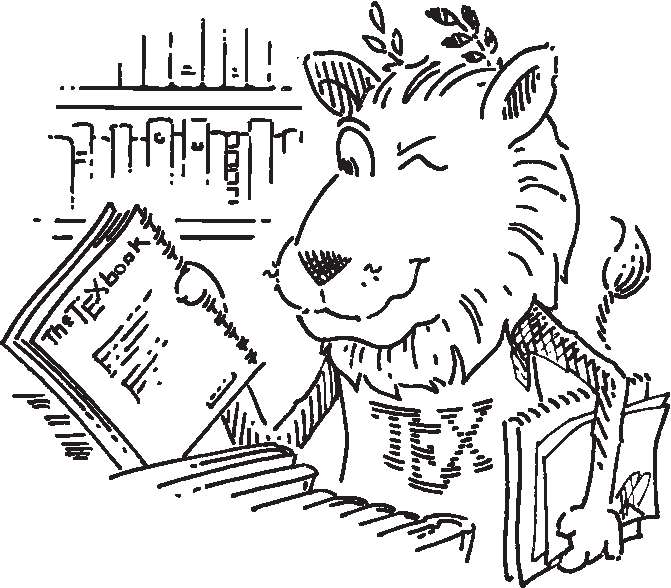
\includegraphics[width=0.6\textwidth]{imgs/ctanlion}
	\fonte{Duane Bibby, diponibilizado em \url{www.ctan.org/lion}}
\end{figure}


 Só é importante se atentar para dois detalhes: os títulos das figuras, que devem vir antes do \texttt{inludegraphics}, e a fonte, que deve ser posicionada após o \texttt{inludegraphics} e pode utilizar o comando pré definido \texttt{fonte}. Exemplo do código para a \autoref{fig:leaoCTAN}:
\begin{lstlisting}[language={[LaTeX]Tex}]
\begin{figure}
	\centering
	% \caption antes da figura
	\caption{Leão do site CTAN estudando \TeX} 
	\label{fig:leaoCTAN}
	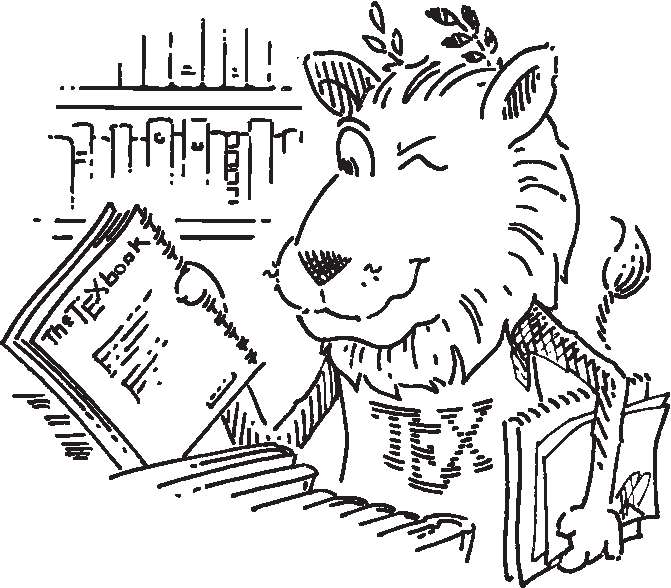
\includegraphics[width=0.6\textwidth]{imgs/ctanlion}
	\fonte{Duane Bibby, diponibilizador por \url{www.ctan.org}}
\end{figure}
\end{lstlisting}



\section{Quadros e Tabelas}\label{sec:tabelasUFLA}

A normalização da UFLA reconhece dois principais tipos de elementos tabulares, tabelas e quadros, com conteúdos e formatos específicos. 

\begin{table}[h]
	\centering
	\caption{Exemplo de Tabela} 
	\label{tab:exemplo2}
	\begin{tabular}{c c c c }
		\hline
		\linhadir{\bf Pessoa} & \linhadir{\bf Livros} & \linhadir{\bf Artigos} & \bf Palestras \\
		\hline
		$p_1$ & 1 & 3 & 4 \\
		$p_2$ & 1 & 3 & 3 \\
		$p_3$ & 1 & 3 & 4 \\
		$p_4$ & 3 & 5 & 2 \\
		\hline 
	\end{tabular}
	\vspace{0.3cm}
	\fonte{original} %Fonte do tabela
\end{table}

Tabelas envolvem principalmente números, utiliza-se linhas horizontais somente no topo, final e cabeçalhos, além disso utiliza-se linhas verticais somente nos cabeçalhos\footnote{Por isso a \autoref{tab:exemplo} não segue o padrão correto.}. Para reduzir o tamanho do código dos cabeçalhos, a classe \texttt{templufla} define do comando \texttt{linhadir}, que adiciona uma linha vertical à direita da célula. Abaixo mostra-se um exemplo do código para a \autoref{tab:exemplo2}:
\begin{lstlisting}[language={[LaTeX]Tex}]
\begin{table}[h]
	\centering
	\caption{Exemplo de Tabela} 
	\label{tab:exemplo2}
	\begin{tabular}{c c c c }
		\hline
		\linhadir{Pessoa}& \linhadir{Livros}& \linhadir{Artigos}& Palestras\\
		\hline
		$p_1$& 1& 3& 4\\
		$p_2$& 1& 3& 3\\
		$p_3$& 1& 3& 4\\
		$p_4$& 3& 5& 2\\
		\hline 
	\end{tabular}
	\vspace{0.3cm}
	\fonte{original} %Fonte do tabela
\end{table}
\end{lstlisting}


Quadros se diferem das tabelas por conterem principalmente dados textuais e suas células serem completamente fechadas. O \autoref{quad:exemplo} é um exemplo de quadro.

\begin{quadro}[h]
\centering
\caption{Opiniões sobre esse template}\label{quad:exemplo}
  \begin{tabular}{|l|p{9cm}|}
    \hline 
    \rowcolor[gray]{.9}
    \bf Nome& \bf Opinião\\
    \hline
    Jão& Desculpe, não posso comentar sobre isso.\\
    \hline
    Joana& Literalmente uma revolução do cinema nacional!\\
    \hline
    Jacquin& Esse autor é a vergonha da profisson!\\
    \hline
    Meu cachorro& Au! Au! Au! $\sim$Sons de papel sendo rasgado.\\
    \hline
    Overleaf& ASSINE, ASSINE O PREMIUM.\\
    \hline
    \end{tabular}
    
    \vspace{0.3cm}
	\fonte{original}
\end{quadro}


\section{Padrão das Referências}

Desde que o padrão descrito na \autoref{sec:Refs} seja seguido e partes importantes do template sejam mantidas, as referências não devem ser um problema. O template já vem configurado para o formato padrão da ABNT, desde que os arquivos \texttt{abntex.*}, o preâmbulo e a chamada dos comandos \texttt{bibliographystyle}, \texttt{citeoption}, \texttt{refencias} e \texttt{bibliography}, próximos ao final do arquivo principal, sejam mantidos.

É comum referências serem um problema e, apesar do \LaTeX\ ajudar muito nisso, o processo ainda pode ser complicado. O pacote \texttt{abntex2} está desatualizado, as correções precisaram ser \emph{hard-coded} e o arquivo principal reflete isso.

\textbf{Então, se você quer que as citações e referências sejam tão simples quanto adicionar um \texttt{bibtex} e usar o comando \texttt{cite}, EU TE SUPLICO, não altere o preâmbulo nem os comandos relacionados às referências no \texttt{tempulfa\_main.tex}.}

Referências sortidas para contribuir para a lista ao final (ignore): \cite{Eco1996,Booth2000,BIB2010,Hexsel2004,Franca2001,Gil2002,Porto2002,Silva2005,UFLA:2015,Moura1998,NBR6023:2002,LeGuin:1987}


\chapter{LISTAS, GLOSSÁRIO E ÍNDICE}\label{sec:listasEGlossario}

O template também inclui a criação dos elementos pré-textuais lista de abreviações (ou, como está no manual, abreviaturas), siglas e símbolos. Além disso, também inclui a criação do glossário e índice.

Todos esses novos elementos, exceto o índice, utilizam o mesmo pacote, \texttt{glossaries}, então, têm comportamento semelhante. Cada ítem deve ser adicionado aos glossários no preâmbulo e, após adicionados, podem ser referenciados no documento com o comando \texttt{gls}. Por exemplo:
	
\begin{figure}[!htb]
	\centering
	\caption{Inserindo ítem no \gls{glo:glossario} e o referindo no texto} %legenda
	\label{fig:exemploglossario1} %rotulo para refencia
	\begin{lstlisting}[language=tex]
\newglossaryentry{glo:glossario}{
	name={glossário}, 
	description={
		Relação de palavras ou expressões técnicas 
		de uso restrito ou de sentido obscuro, 
		utilizadas no texto, acompanhadas das 
		respectivas definições}
	}
		
%\makeglossaries % não é necessario nesse template pois já é chamado na classe
\begin{document}
...
\caption{Inserindo ítem no gls(glo:glossario) e o referindo no texto}
	\end{lstlisting}
	
	\fonte{original}
\end{figure}

O comando \textit{\textbf{gls}} escreve o nome do ítem quando é usado. Para que outro valor seja escrito, ou até para que nada seja escrtio, pode-se utilizar o comando \texttt{glslink}:
\begin{lstlisting}[language=tex]
	\glslink{<rótulo>}{<texto alternativo>}
\end{lstlisting}

É recomendável separar as adições aos glossários em arquivos para melhor organização e reduzir o tamanho do preâmbulo. Nesse template, cada glossário tem seu próprio arquivo, adicionado ao projeto via comandos \texttt{loadglsentries}, e os arquivos têm sua própria pasta. Essa organização pode ser alterada, desde que a mudança seja refletida no preâmbulo.

\newpage
Abaixo listamos o formato para a adição de ítens em cada glossário:

\begin{alineas}
	\item \textbf{abreviaturas}: Adicionar uma abreviatura é simples e a sintaxe é relativamente fixa.\\ Um exemplo para a abreviatura de \gls{jan}:
		\begin{lstlisting}[language=tex]
\newabbreviation{jan} % rótulo
{jan.}% forma abreviada
{Janeiro} % forma completa
...
... Um exemplo para a abreviatura de \gls{jan}:
		\end{lstlisting}
	
	\item \textbf{siglas}: Adicionar siglas é igualmente simples.\\ 
	Um exemplo para a sigla \gls{abnt}:
	\begin{lstlisting}[language=tex]
\newacronym{abnt} % rótulo
{ABNT} % sigla
{Associação Brasileira de Normas Técnicas} % nome completo
...
... Um exemplo para a sigla \gls{abnt}:
	\end{lstlisting}
	
	\item \textbf{símbolos}: Adicionar símbolos é um pouco mais complicado, já que necessita de uma descrição. Como a lista é por ordem de uso, \gls{gama} deve aparecer antes de \gls{alfa}\\ 
	Um exemplo para o símbolo \gls{gama}:
	\begin{lstlisting}[language=tex]
\newglossaryentry{gama}{
	name={$\gamma$}, % o símbolo em questão
	description={Um número gama}, % descrição do símbolo
	type={symbols}} % indicador que é um símbolo
...
... Um exemplo para o símbolo \gls{gama}:
	\end{lstlisting}
	
	\item \textbf{glossário}: Adicionar termos no glossário é igual ao exemplo mostrado antes.\\
	Nesse caso, no entanto, adicionamos uma \emph{tag} \LaTeX\ antes do nome, então temos que adicionar o valor "\emph{sort}", para que a ordenação seja correta.
	Um exemplo para o termo \gls{llm}:
	\begin{lstlisting}[language=tex]
\newglossaryentry{llm}{
	name={\emph{large language model}}, % o nome do termo
	description={Grande model de 
		linguagem. Ex:DeepSeek-R1}, % descrição do termo
	sort={large language model}} % chave para ordenação
...
... Um exemplo para o termo \gls{llm}:
	\end{lstlisting}
	
	\item \textbf{índice}: Adicionar termos ao índice é o mais fácil de todos. Para adicionar um índice, basta utilizar o comando \emph{index}. Caso algum índice tiver um pai(ou mãe), basta adicionar o delimitador ``!''.\\
	Um exemplo para os termos conjunto\index{Conjunto}, conjunto aberto\index{Conjunto!aberto} e conjunto fechado\index{Conjunto!fechado}:
	\begin{lstlisting}[language=tex]
...Um exemplo para os termos conjunto\index{Conjunto},
conjunto aberto\index{Conjunto!aberto} e conjunto 
fechado\index{Conjunto!fechado}:
	\end{lstlisting}
	
\end{alineas}

Para mais informações sobre como usar esses pacotes, consulte as documentações oficiais do \texttt{glossaries}\footnote{https://ctan.org/pkg/glossaries?lang=en} e do \texttt{imakeidx}\footnote{https://ctan.org/pkg/imakeidx}.

%\chapter{ELABORAÇÃO DE REFERÊNCIAS}
\label{cap:elementos5}

Referência é um conjunto padronizado de elementos descritivos, retirados de um documento que permite sua identificação individual, seguindo normas vigentes, permitindo, dessa forma, que as informações contidas no texto possam ser efetivamente comprovadas, quando necessário. Esses elementos devem ser apresentados em sequência padronizada e são extraídos do documento que estiver sendo referenciado.

Para a elaboração das referências é necessária a identificação dos elementos essenciais, que são informações indispensáveis à identificação do documento. Estão estritamente vinculados ao suporte documental e variam, portanto, conforme o tipo de obra. Se necessário, também é possível utilizar elementos complementares para melhor identificação da obra. Contudo, ``ao optar-se pela utilização de elementos complementares, estes devem ser incluídos em todas as referências daquela lista'', conforme estabelece a NBR 6023 \cite{NBR6023:2002}. As referências podem ser dispostas:

\begin{enumerate}[a)]
  \item	 no rodapé;
  \item	 no final do texto ou do capítulo;
  \item	 em lista de referências;
  \item	 antecedendo resumos, resenhas e recensões.
\end{enumerate}

A lista de referências tem a finalidade de apresentar ao leitor as obras e os autores que serviram de base para a elaboração do trabalho. As referências oferecem uma ideia geral de toda a documentação consultada e, ainda, oferece a possibilidade de aprofundamento do tema mediante consulta às fontes originais. 

Relacionam-se as referências em lista própria. São apresentadas no final do trabalho, em ordem alfabética, com entrada única (sobrenome de autor, entidade autora e título, em letras maiúsculas) e a alfabetação deverá ser de acordo com a NBR 6033 \cite{NBR6033:1989}. Em caso de trabalhos em formato de capítulos e artigos, deverá haver lista própria no final dos mesmos. Aparece sob o título de Referências, em maiúsculas, centralizado e negrito. As referências são alinhadas à margem esquerda do texto, digitadas com espaço simples entre as linhas. ``As referências, ao final do trabalho, devem ser separadas entre si por um espaço simples em branco'' \cite[p.10]{NBR14724:2011}.

A pontuação segue padrões internacionais e deve ser uniforme. Para melhor padronização dos trabalhos, na UFLA utiliza-se o recurso tipográfico negrito para destaque dos dados, de acordo com cada tipo de material usado (título do livro, da tese, do periódico e outros). Para a entrada de autores, indica o último sobrenome, todo em letras maiúsculas, seguido do(s) prenome(s) e outros sobrenomes, abreviado(s) por suas iniciais. Deverá haver espaço entre as iniciais de sobrenomes, volume, número, e páginas. Para a elaboração das referências, consultar a NBR 6023 \cite{NBR6023:2002}.

As dissertações e teses em formato de artigos encaminhados e/ou aceitos para publicação poderão manter as referências elaboradas conforme as normas do periódico científico. 


\section{Pontuação}

Os vários elementos de uma referência devem ser separados entre si por uma pontuação uniforme, como explicado a seguir:

\begin{enumerate}[a)]
  \item	 \textbf{Ponto} (.): usa-se o ponto, seguido de espaço, após a indicação dos seguintes elementos: nome(s) do(s) autor(es), título da obra, edição, imprenta (local, editora e data), número de páginas e/ou  volumes. Após abreviaturas de prenomes de autor (SOARES, J. A.) e número de edição (3. ed.), usa-se o ponto com espaço;
  \item	 \textbf{Ponto e vírgula} (; ): usa-se o ponto e vírgula, seguido de espaço, para separar autores entre si (SOARES, J. A.; LOPES, M. A.; ANDRADE, M. A. de.);
  \item	 \textbf{Vírgula} (,): usa-se a vírgula, seguida de espaço, para separar sobrenome do nome do autor (SOARES, J. A.); para separar o nome do editor da data de publicação e na separação da indicação de volume, número de fascículo e data na referência de artigo de periódico (v. 3, n. 4, abr. 1998); também na separação de volume e página (v. 3, 364 p.) ou volume, capítulo e página (v. 3, cap. 1, p. 28-56);
  \item	 \textbf{Dois pontos} (:): dois pontos, seguidos de espaço, são usados para separar o título do subtítulo (Brasília: a cidade e o homem) e entre o local de publicação e nome do editor (São Paulo: Atlas);
  \item	 \textbf{Hífen} (-): usa-se o hífen para ligar página inicial e final de parte referenciada (p. 10-38); 
  \item	 \textbf{Barra} (/): ligam-se por barra transversal os elementos do período coberto pelo fascículo referenciado, quando este constitui uma só unidade, sendo volume, número do fascículo, mês e ano (v. 9/10, n. 1/4, jan./dez., 2013/2014); 
  \item	 \textbf{Colchetes} ([ ]):  indicam-se entre colchetes os elementos não extraídos da folha de rosto da obra referenciada e para indicar ausência  dos elementos. Ex: [S.l.] \textit{sine} loco = sem local; [s.n.] \textit{sine nomine} = sem nome; [1993?] data provável de publicação;
  \item	 \textbf{Reticências} (...): empregada quando se faz supressão de parte do título. Na referenciação, por exemplo, de anais de congresso, simpósio e outros eventos sem título específico, indica-se o título apenas por \textbf{Anais}..., \textbf{Resumos}..., etc;
  \item	 \textbf{Travessão} (\rule{1cm}{0.4pt}): Eventualmente, o(s) nome(s) do(s) autor(es) de várias obras referenciadas sucessivamente, na mesma página, pode(m) ser substituído(s), nas referências seguintes à primeira, por um traço sublinear (equivalente a seis espaços) e ponto.
\end{enumerate}

\begin{exemplomanual}
\textbf{Exemplos}:\\
\begin{singlespace}
SOUZA, R. J. de et al. \textbf{Cultura da beterraba}: cultivo convencional e cultivo orgânico. Lavras: UFLA, 2003. 37 p. (Textos acadêmicos, 34).\\*
%\newline
%\newline

\rule{1cm}{0.4pt}. \textbf{Cultura da cenoura}. Lavras: UFLA, 2002. 68 p. (Textos acadêmicos, 22).
\end{singlespace}
\end{exemplomanual}


\section{Aspecto tipográfico}

Deve-se utilizar o mesmo tipo e tamanho de caractere do texto. Na UFLA, padronizou-se a utilização do \textbf{negrito} nos títulos em destaque nas referências.

Nomenclatura científica de gêneros e espécies devem ser grafados em \textit{itálico}, observando-se para que não ocorra divisão silábica, por se tratar de nomes latinos.  Exemplo: \textbf{Bibliografia do milho}, \textit{Zea mays}.


\section{Apresentação e transcrição dos elementos}

Os elementos devem ser apresentados e descritos conforme estabelecido em 7.3.1 a 7.3.6.


\subsection{Autor}

O autor constitui a entrada principal da referência. Quando este não é identificado na publicação referenciada, faz-se a entrada pelo título.

Identificam-se os autores como \textbf{pessoal} (pessoa física), \textbf{corporativo} (órgãos governamentais, empresas, congressos, etc.) e \textbf{autor desconhecido} (anônimo) quando não identificado na publicação referenciada.


\subsubsection{Autor pessoal}

Indicam-se os autores pessoais com a entrada pelo último sobrenome, em letras maiúsculas, separados por vírgula e espaço do(s) prenome(s) abreviado(s). Os autores são separados entre si por ponto e vírgula, seguido de espaço. Outras informações sobre entrada de nomes estrangeiros no Anexo A.

\begin{exemplomanual}
\textbf{Exemplo}:
LOPES, J. P.; MELO, P. N. de.
\end{exemplomanual}

O nome do autor é transcrito na referência, tal como está apresentado na publicação, com prenomes abreviados. Ex.: BILAC, O. (para Olavo Bilac) ou, BILAC, O. B. M. dos G. (para Olavo Braz Martins dos Guimarães Bilac).

\begin{enumerate}[a)]
  \item  \textbf{Até três autores}: indicam-se os autores na mesma ordem apresentada na publicação.

\begin{exemplomanuallista}
\textbf{Exemplo}:\\
Apenas um autor: ARAÚJO, J. A. de.\\
Dois autores: LOPES, J. P.; MELO, P. N. de.\\
Três autores: SOUSA, M. A.; SOARES, M. A.; MELO, P. N. de.
\end{exemplomanuallista}
  
  \item  \textbf{Mais de três autores}: segundo a NBR6023 \cite{NBR6023:2002} quando existirem mais de três autores, indica-se apenas o primeiro, acrescentando-se a expressão ``et al.'' (sem itálico).

  \begin{exemplomanuallista}
  \textbf{Exemplo}:\\
  SOUZA, P. A. et al.
  \end{exemplomanuallista}
\end{enumerate}


\subsubsection{Responsabilidade intelectual}

Quando houver indicação explícita de responsabilidade pelo conjunto da obra, em coletâneas de vários autores, a entrada deve ser feita pelo nome do responsável, seguida da abreviação, no singular, do tipo de participação (organizador, compilador, editor, coordenador etc.), entre parênteses.

\begin{exemplomanual}
\textbf{Exemplos}:\\
CUNHA, J. A. (Coord.).\\
ALMEIDA, M. P.; SOARES, M. A.; ALMEIDA, A. (Org.).\\
FERRI, M. G. (Ed.).
\end{exemplomanual}


\subsubsection{Autor corporativo}

Designa-se autor corporativo qualquer entidade coletiva responsável pela autoria de uma publicação (ver também Anexo B - Entrada para autores corporativos).

A entidade coletiva, quando responsável pela autoria da publicação referenciada, é transcrita em letras maiúsculas. A identificação geográfica, quando não fizer parte do nome da instituição, é acrescentada entre parênteses.

\begin{exemplomanual}
\textbf{Exemplos}:\\
BIBLIOTECA NACIONAL (Brasil).\\
INSTITUTO BRASILEIRO DE GEOGRAFIA E ESTATÍSTICA (Rio de Janeiro, RJ).
\end{exemplomanual}

\begin{enumerate}[a)]
  \item  \textbf{Órgãos governamentais}: os órgãos dos Poderes Executivo, Legislativo e 
   Judiciário, entram pelo nome do local de sua jurisdição (país, estado ou   município). Chefes de estado, forças armadas, embaixadas, consulados, e   delegações internacionais, entrar pelo país seguido do órgão subordinado.
   
\begin{exemplomanuallista}
\textbf{Exemplos}:\\
BRASIL. Ministério da Educação e do Desporto.\\
BRASIL. Tribunal Superior Eleitoral.\\
MINAS GERAIS. Secretaria de Agricultura.
\end{exemplomanuallista}

  \item  \textbf{Termos que constituem entrada principal}: (ver também \textbf{Anexo B} – 
    Entrada para autores corporativos, item 1).
    
\begin{exemplomanuallista}
\textbf{Exemplos}:\\
CÂMARA BRASILEIRA DO LIVRO (Rio de Janeiro, RJ). \\
COMISSÃO DE FERTILIDADE DO SOLO DO ESTADO DE MINAS GERAIS.
\end{exemplomanuallista}

  \item  \textbf{Unidades}: unidades subordinadas administrativamente ao órgão superior faz-se a entrada pelo órgão superior em caixa alta seguido, após ponto, da unidade e identificação geográfica, quando necessária. Os termos que implicam em subordinação administrativa estão apresentados no \textbf{Anexo B}, item 2.
  
\begin{exemplomanuallista}
\textbf{Exemplos}:\\
UNIVERSIDADE FEDERAL DE LAVRAS. Biblioteca Universitária.\\
EMBRAPA. Centro Nacional de Pesquisa de Gado de Leite.
\end{exemplomanuallista}

  \item  \textbf{Sigla}: quando uma entidade é melhor conhecida por sua sigla, dar preferência a esta forma seguida da identificação geográfica.
  
\begin{exemplomanuallista}  
\textbf{Exemplos}:\\
EMBRAPA (Brasília, DF). \\
FAO (Roma, Itália).
\end{exemplomanuallista}
\end{enumerate}

Não é recomendado o uso de sigla quando se tratar de comissões, congressos, conselhos (exceção: CNPq), escolas, faculdades, universidades, órgãos subordinados administrativamente e entidades governamentais.


\subsubsection{Autor desconhecido}

Em caso de autoria desconhecida, entra-se pelo título. O termo anônimo não deve ser usado em substituição ao nome do autor. A primeira palavra do título deve ser transcrita em caixa alta.

\begin{exemplomanual}  
\textbf{Exemplos}:\\
ESTUDOS filosóficos: homenagem a Serafim da Silva Neto.\\
A PREVIDÊNCIA social no Brasil.
\end{exemplomanual}  


\subsection{Título}

O título é transcrito como está redigido na publicação referenciada, colocar somente em letras maiúsculas a letra inicial e as iniciais de nomes próprios. A supressão de parte do título só deve ocorrer para títulos demasiadamente longos, sem incidir sobre as primeiras palavras para não ocorrer alteração do sentido. Faz-se a supressão com o uso de reticências. Suprime-se o subtítulo quando este fornecer informação irrelevante à compreensão do título.

\begin{enumerate}[a)]
  \item  \textbf{Título principal de livros, teses, folhetos e similares}: transcreve-se o título em negrito e acrescenta-se o subtítulo (sem negritar), separado por dois pontos;

\begin{exemplomanuallista}  
\textbf{Exemplo}:\\
\textbf{Agroecologia}: bases científicas para a agricultura alternativa.
\end{exemplomanuallista}

  \item  \textbf{Título de periódico}: transcrever o título de periódico ou seriado por extenso, em negrito, quando se tratar de referência de artigo (ver 7.5.5.3 a 7.5.5.5);

\begin{exemplomanuallista}  
\textbf{Exemplo:\\
Pesquisa Agropecuária Brasileira.}
\end{exemplomanuallista}  

No caso de periódico referenciado como um todo, o título é sempre o primeiro elemento da referência, tanto para a referência de número especial como de coleção completa (ver 7.5.5.1), sendo transcrito por extenso e em caixa alta.

\begin{exemplomanuallista}
\textbf{Exemplo}:\\
PESQUISA AGROPECUÁRIA BRASILEIRA.
\end{exemplomanuallista}

  \item  \textbf{Acréscimo ao título}: títulos em língua de difícil acesso (não latinas) pode-se acrescentar o título traduzido, após título em língua original, entre colchetes;
  
Outros acréscimos apresentados na publicação referenciada, quando considerados essenciais, podem ser indicados após o título.

\begin{exemplomanuallista}
\textbf{Exemplo}:\\
\begin{singlespace}
PENA, L. C. M. \textbf{Comédias de Martins Pena}. Edição crítica por Darcy Damasceno com a colaboração de Maria Filgueiras.
\end{singlespace}
\end{exemplomanuallista}

  \item  \textbf{Títulos de congressos e outros eventos}: quando não há um título específico e são tratados genericamente como anais do congresso... resumos do congresso..., etc., indica-se o título apenas por \textbf{Anais}...,  \textbf{Resumos}..., etc., seguido de reticências (ver 7.5.6 e 7.5.7);
  
  \item  \textbf{Publicações traduzidas}: acrescenta-se o nome do tradutor após o título e em nota especial acrescenta-se o título original. Ambos os acréscimos são precedidos da expressão ``Tradução de''. Esse recurso deve ser utilizado somente em casos especiais para diferenciar uma obra da outra
  
\begin{exemplomanuallista}
\textbf{Exemplo}:\\
\begin{singlespace}
CHRISMAN, C. L. \textbf{Neurologia dos pequenos animais}. Tradução de André Luís Montagnini et al. São Paulo: Roca, 1985. 432 p. Tradução de: Problems in small animal neurology.
\end{singlespace}
\end{exemplomanuallista}

  \item  \textbf{Documento sem título}: quando o documento não possuir título, deve-se atribuir uma palavra ou frase para identificar o documento, entre colchetes.

\begin{exemplomanuallista}
\textbf{Exemplo}:\\
\begin{singlespace}
SIMPÓSIO BRASILEIRO DE AQUICULTURA, 1., 1978, Recife.[\textbf{Trabalhos apresentados}]. Rio de Janeiro: Academia Brasileira de Ciências, 1980. ii, 412 p.
\end{singlespace}
\end{exemplomanuallista}
\end{enumerate}


\subsection{Edição}

 Segundo a NBR 6023 \cite{NBR6023:2002} ``Quando houver uma indicação de edição, esta deve ser transcrita, utilizando-se abreviaturas dos numerais ordinais e da palavra edição, ambas na forma adotada na língua do documento''. 

\begin{exemplomanual}
\textbf{Exemplos}:

\begin{enumerate}[a)]
  \item  2. ed. (segunda edição, português, espanhol);
  \item  2nd ed. (segunda edição em língua inglesa);
  \item  3rd ed. (terceira edição em língua inglesa);
  \item  11th ed. (décima primeira edição em língua inglesa);
  \item  2. Aufl. (segunda edição em língua alemã);
  \item  4. ed., corr. y aum. (quarta edição em língua espanhola);
  \item  4. éd. (quarta edição em língua francesa);
  \item  3ª ed. (terceira edição em italiano).
\end{enumerate}
\end{exemplomanual}

Os acréscimos à edição como revista, aumentada, ampliada, atualizada, devem ser indicados de forma abreviada, com espaço.

\begin{exemplomanual}
\textbf{Exemplos}:

\begin{enumerate}[a)]
  \item  2. ed. rev. (segunda edição revista);
  \item  2. ed., rev. e aum. (segunda edição revista e aumentada);
  \item  2. ed., rev. e atual. (segunda edição revista e atualizada).
\end{enumerate}
\end{exemplomanual}


\subsection{Local (cidade)}

O local apresentado na referência é a cidade onde a publicação foi editada. Este deve ser transcrito na língua da publicação, de forma completa e por extenso como Rio de Janeiro (e não Rio), Belo Horizonte (e não BH), London (e não Londres).

No caso de homônimos, acrescenta-se o nome do estado ou país.

\begin{exemplomanual}
\textbf{Exemplos}:

\begin{enumerate}[a)]
  \item  San Juan, Chile;
  \item  San Juan, Puerto Rico;
  \item  Viçosa, MG;
  \item  Viçosa, AL;
  \item  Viçosa, RJ.
\end{enumerate}
\end{exemplomanual}

Havendo mais de um local de publicação, transcreve-se o primeiro ou o que estiver em destaque. Quando o local não aparece na publicação, mas pode ser identificado, indica-se entre colchetes. Sendo impossível determinar o local, adota-se a abreviatura [S.l.] (\textit{sine loco}) = sem local, entre colchetes.


\subsection{Editora}

O nome da editora é transcrito após o local, precedido de dois pontos seguido de espaço. No caso de editores com nomes pessoais, indicam-se os prenomes por iniciais maiúsculas, seguidos de ponto e sobrenome por extenso, suprimindo-se os elementos que designam a natureza jurídica ou comercial, tais como: ``Company'', ``Ltda'', ``Sons'', ``Livraria'', ``Papelaria'', ``Lithografia'', ``Typographia'', etc ``desde que sejam dispensáveis para a identificação'' conforme a NBR 6023 \cite{NBR6023:2002}.

\begin{exemplomanual}
\textbf{Exemplos}:

\begin{enumerate}[a)]
  \item  J. Wiley - (não John Wiley \& Sons);
  \item  J. Olympio (não José Olympio Editora);
  \item  F. Alves (não Livraria Francisco Alves);
  \item  J. Zahar (não Jorge Zahar Editor);
  \item  M. Fontes (não Editora Martins Fontes).
\end{enumerate}
\end{exemplomanual}

Quando houver duas editoras, as duas são indicadas, com suas respectivas cidades. Havendo três ou mais, indica-se a primeira ou a que estiver em destaque.

\begin{exemplomanual}
\textbf{Exemplo}:\\
\begin{singlespace}
ALFONSO-GOLDFARB, A. M.; MAIA, C. A. (Coord.) \textbf{História da ciência}: o mapa do conhecimento. Rio de Janeiro: Expressão e Cultura; São Paulo: EDUSP, 1995. 968 p. (América 500 anos, 2).
\end{singlespace}
\end{exemplomanual}

Não se indica o editor, quando este é o próprio autor.

\begin{exemplomanual}
\textbf{Exemplo}:\\
\begin{singlespace}
UNIVERSIDADE FEDERAL DE VIÇOSA. Catálogo de graduação.\\
1994-1995. Viçosa, MG, 1994. 385 p.
\end{singlespace}
\end{exemplomanual}

Na ausência de editor, indica-se [s.n.] (\textit{sine nomine}) = sem editora, entre colchetes. Quando estiverem ausentes o local e o editor indica-se [S.l.: s.n.], entre colchetes.

\begin{exemplomanual}
\textbf{Exemplo}:\\
\begin{singlespace}
FRANCO, I. Discursos: de outubro de 1992 a agosto de 1993. Brasília, DF: [s.n.], 1993. 107 p.
\end{singlespace}
\end{exemplomanual}


\subsection{Data}

Transcreve-se o ano de publicação em algarismos arábicos, precedido por vírgula e espaço. Não sendo possível determinar a data de publicação, distribuição, impressão ou copyright, indica-se uma data aproximada, entre colchetes:

\begin{exemplomanual}
\textbf{Exemplos}:\\*

%\newline
a) [1983?] para data provável;\\*
b) [ca. 1960] para data aproximada; (ca = cerca de);\\*
c) [198-] para década certa;\\*
d) [18--] para século certo;\\*
e) [18--?] para século provável.
\end{exemplomanual}

Para publicações periódicas em curso de publicação, indica-se a data inicial seguida de hífen (1978-) (ver 7.5.5.1 alínea a). Também são ligados por hífen as datas extremas de publicação periódica encerrada (1959-1985) (ver 7.5.5.1 alínea b).

Faz-se a indicação de mês de forma abreviada no idioma original da publicação, conforme lista de abreviaturas apresentadas no Anexo C. Meses com quatro ou menos letras são transcritos por extenso.

Quando, em lugar dos meses, a publicação apresentar as estações ou divisão do ano em trimestre, semestre, etc., transcrevem-se os primeiros e abreviam-se os últimos, conforme a NBR 6023 \cite{NBR6023:2002}.

\begin{exemplomanual}
\textbf{Exemplos}:

\begin{enumerate}[a)]
  \item  Summer 1998;
  \item  2. trim. 1998.
\end{enumerate}
\end{exemplomanual}

Quando mais de um trabalho do mesmo autor, publicado na mesma data são apresentados numa lista bibliográfica, estes devem ser identificados por letras minúsculas após a data.

\begin{exemplomanual}
\textbf{Exemplos}:

\begin{enumerate}[a)]
  \item[a)] SOUSA, A. S. Ocorrência... 1980a;
  \item[b)] SOUSA, A. S. Produção... 1980b. 
\end{enumerate}
\end{exemplomanual}


\section{Descrição física}

A indicação de paginação, volumes e notas complementares deve ser feita conforme indicado em 7.4.1 e 7.4.2.


\subsection{Número de páginas e volumes}

Quando se tratar de referência de uma publicação no todo, indica-se o total de páginas seguido da abreviatura ``p.'' com espaço (ex.: 260 p.); se a publicação tem mais de um volume, indica-se o número destes, seguido de abreviatura ``v.'' com espaço (ex.: 3 v.); na referência de um dos volumes da coleção, indica-se o número do volume precedido da abreviatura ``v.''(ex.: v. 2). Quando indicado(s) o(s) volume(s) de obras referenciadas no todo, a indicação de número de páginas é opcional.

Em referência de capítulos ou partes de monografias e artigos de periódicos indica-se a página inicial e final da parte, precedido da abreviatura ``p.'' com espaço após a letra (\textbf{exemplo}: p. 34-40). Quando há volume, capítulo, fascículo, estes precedem à indicação da página (\textbf{exemplo}: v. 3, n. 2, p. 38-46, para artigo de periódico) e (v. 2, cap. 3, p. 69-75, para parte de monografia).

Quando a publicação não for paginada, indica-se: não paginado, ou quando for paginada irregularmente, indica-se: paginação irregular.

Pode-se registrar o número da última página, folha ou coluna de cada sequência, respeitando-se a forma encontrada (letras, algarismos romanos e arábicos) NBR 6023 \cite{NBR6023:2002}.

\begin{exemplomanual}
\textbf{Exemplo}:\\
\begin{singlespace}
JAKUBOVIC, J.; LELLIS, M. \textbf{Matemática na medida certa, 8. série}:
livro do professor. 2. ed. São Paulo: Scipione, 1994. 208, xxi p.
\end{singlespace}
\end{exemplomanual}


\subsection{Notas}

\begin{enumerate}[a)]
  \item  \textbf{Série e coleções}: títulos de série ou coleções são indicados com iniciais de palavras em letra maiúscula, entre parênteses, após a indicação da paginação, e seguido do número ou volume, quando houver, separados por vírgula.

\begin{exemplomanuallista}
\textbf{Exemplos}:\\
(Série Técnico-científica, 39)\\
(Visão do futuro, v. 41)\\
(Texto para discussão, n. 4)
\end{exemplomanuallista}

Quando se tratar de duas ou mais notas de série, separá-las por ponto e vírgula.

  \item  \textbf{Teses, dissertações, trabalho de conclusão de curso}: transcreve-se o termo ``tese'', ``dissertação'', ``trabalho de conclusão de curso'' como apresentado no documento original, seguido do nome do curso, entre parênteses.
   
\begin{exemplomanuallista}
\textbf{Exemplos}:\\
Dissertação (Mestrado em Ciência dos Alimentos)\\
Tese (Doutorado em Agronomia/Fitotecnia)\\
Trabalho de Conclusão de Curso (Especialização)
\end{exemplomanuallista}

  \item  \textbf{Outras notas}: notas especiais, inclusive aquelas que esclarecem sobre forma da publicação, tais como: mimeografado, apostila, folder, resenha, resumo, fac-símile, no prelo, CD-ROM etc., são apresentadas no final da descrição da publicação, sem uso de parênteses.
\end{enumerate}


\section{Modelos de referências}

Nesta seção exemplificam-se os formatos das referências relativo a cada tipo de documento considerado no todo e em parte.



\subsection{Monografia considerada no todo}

Segundo a NBR 6023 \cite[p.3]{NBR6023:2002}, ``inclui livro e/ou folheto/manual, guia, catálogo, enciclopédia, dicionário, etc.) e trabalhos acadêmicos (tese, dissertação, entre outros)''.

\begin{flushleft}
  \fbox{
    \parbox{\textwidth-0.5cm}{AUTOR. \textbf{Título}. Edição. Local (cidade): Editora, data.}
    }
\end{flushleft}
 
\noindent\rule{12.5cm}{0.4pt}
\begin{flushleft}
\textbf{Exemplos:}

\begin{singlespace}
BRASIL. Ministério da Justiça. \textbf{Relatório de atividades}. Brasília, DF,
1993. 28~p.
\newline
\newline
CHALFUN, N. N. J. \textbf{A cultura da figueira}. Lavras: Ed. UFLA, 2012. 342 p. 
\newline
\newline
COMISSÃO DE FERTILIDADE DO SOLO DO ESTADO DE MINAS GERAIS. \textbf{Recomendações para o uso de corretivos e fertilizantes em Minas Gerais}: 5ª aproximação. Viçosa, MG, 1999. 359 p.
\newline
\newline
MOREIRA, F. M. S.; SIQUEIRA, J. O. \textbf{Microbiologia e bioquímica do solo}. 2. ed. Lavras: Ed. UFLA, 2006. 729 p. 
\newline
\newline
NOVA Enciclopédia Barsa.  Rio de Janeiro: Encyclopaedia Britannica do Brasil, 1998. 20 v.
\newline
\newline
SALVADOR, S. C. et al. \textbf{Principais intoxicações em cães e gatos}. Lavras: Ed. UFLA, 2005. 45 p. (Textos acadêmicos, 50).
\newline
\newline
SÃO PAULO (Estado). Secretaria do Meio Ambiente. \textbf{Diretrizes para a política ambiental do Estado de São Paulo}. São Paulo, 1993. 35 p.
\newline
\newline
SILVA, F. M. da; ALVES, M. de C. \textbf{Cafeicultura de precisão}. Lavras: Ed. UFLA, 2013. 227 p.
\newline
\newline
SOUZA, R. J. de; MACÊDO, F. S. (Coord.). \textbf{Cultura do alho}: tecnologias modernas de produção. Lavras: Ed. UFLA, 2009. 181 p.
\end{singlespace}
\end{flushleft}
\noindent\rule{12.5cm}{0.4pt}

Para trabalhos acadêmicos:

\begin{flushleft}
\begin{singlespace}
  \fbox{
    \parbox{\textwidth-0.5cm}{AUTOR. \textbf{Título}. Data do depósito. N\textsuperscript{\underline{o}} de páginas ou folhas. Tipo de trabalho (Titulação)-Instituição, local, data de defesa.}
    }
\end{singlespace}
\end{flushleft}

\begin{exemplomanual}
\textbf{Exemplo:}\\
\begin{singlespace}
REIS, M. V. dos. \textbf{Gene expression profiles in roses under stress conditions}. 2014. 101 p. Tese (Doutorado em Fisiologia Vegetal)–Universidade Federal de Lavras, Lavras, 2014.
\end{singlespace}
\end{exemplomanual}

\subsection{Monografias consideradas no todo em meio eletrônico}

Inclui os mesmos itens indicados em 7.5.1, em meio eletrônico (disquetes, CD-ROM, online etc.).

As referências devem obedecer aos padrões indicados para os documentos monográficos no todo, acrescidas das informações relativas à descrição física do meio eletrônico NBR6023 \cite[p.4]{NBR6023:2002}.

\begin{exemplomanual}
\begin{singlespace}
\textbf{Exemplo}:\\
DEITEL, H. M.; DEITEL, P. J. \textbf{Java}: como programar. São Paulo: Pearson Prentice Hall, 2006. 1 CD ROM.
\end{singlespace}
\end{exemplomanual}

\begin{quote}
Quando se tratar de obras consultadas online, também são essenciais as informações sobre o endereço eletrônico, apresentado entre os sinais < >, precedido da expressão Disponível em: e a data de acesso ao documento, precedida da expressão Acesso em:, opcionalmente acrescida dos dados referentes a hora, minutos e segundos NBR 6023 \cite[p.4]{NBR6023:2002}.
\end{quote}

A NBR6023 \cite{NBR6023:2002} recomenda que não sejam referenciados os materiais eletrônicos de curta duração nas redes.

\begin{exemplomanual}
\textbf{Exemplo}:\\
\begin{singlespace}
ALBUQUERQUE, E. M. et al. \textbf{Global interactions between firms and universities: global innovation networks as first steps towards a global innovation system}.  Belo Horizonte: UFMG, 2011. (Texto para discussão, 419). Disponível em: \url{http://www.cedeplar.ufmg.br/pesquisas/td/TD\%20419.pdf}. Acesso em: 21 nov. 2013.
\end{singlespace}
\end{exemplomanual}


\subsection{Parte de monografia}

Segundo a NBR6023 \cite[p.4]{NBR6023:2002} ``inclui capítulo, volume, fragmento e outras partes de uma obra, com autor(es) e/ou título próprios''.

\begin{flushleft}
\begin{singlespace}
  \fbox{
    \parbox{\textwidth-0.5cm}{AUTOR DA PARTE REFERENCIADA. Título da parte referenciada. In: AUTOR DA OBRA. \textbf{Título da obra}. Edição. Local: Editora, data. N\textsuperscript{\underline{o}} do volume, n.º do capítulo e/ou página inicial e final da parte referenciada.}
    }
\end{singlespace}
\end{flushleft}


\subsubsection{Autor da parte referenciada igual ao autor da obra}

\begin{exemplomanual}
\textbf{Exemplo}:\\
\begin{singlespace}
RESENDE, M. et al. Substituição isomórfica em goethita, caulinita e hematita. In: \rule{1cm}{0.4pt}. \textbf{Minerologia de solos brasileiros}: interpretação e aplicações. 2. ed., rev. e ampl. Lavras: Ed. UFLA, 2011. cap. 6, p. 133-134.
\end{singlespace}
\end{exemplomanual}


\subsubsection{Autor da parte referenciada diferente do autor da obra}

\begin{exemplomanual}
\textbf{Exemplo}:\\
\begin{singlespace}
OLIVERIA, A. R. de. Práticas de sustentabilidade, acessibilidade e conservação da biodiversidade no Jardim Botânico do Rio de Janeiro. In: ALVES, S. F. N. da S.; REIS, S. N.; PAIVA, P. D. de O. (Org.). \textbf{Coletânia simpósios de paisagismo}: 2002-2008. Lavras: Ed. UFLA, 2009. p. 44-52.
\end{singlespace}
\end{exemplomanual}


\subsection{Parte de monografia em meio eletrônico}

As referências devem ser feitas conforme indicado em 7.5.3 (Parte de monografia) acrescentando-se as informações relativas à descrição física do meio eletrônico (CD-ROM, DVD, online). Quando se tratar de obras consultadas online, deve-se indicar o endereço eletrônico e a data de acesso, conforme explicado em 7.5.2.

\begin{exemplomanual}
\textbf{Exemplo}:\\
\begin{singlespace}
FERREIRA, D. D. et al. Exploiting higher-order statistics information for power quality monitoring. In: EBERHARD, A. \textbf{Power quality}. New York: Intech, 2011. cap. 17, p. 346-362. Disponível em:
\url{http://repositorio.ufla.br/jspui/handle/1/638}.  Acesso em: 13 jun. 2014.
\end{singlespace}
\end{exemplomanual}


\subsection{Publicação periódica}

Segundo a NBR 6023 \cite[p.5]{NBR6023:2002}

\begin{quote}
Inclui a coleção como um todo, fascículo ou número de revista, número de jornal, caderno etc. na íntegra, e a matéria existente em um número, volume ou fascículo de periódico (artigos científicos de revistas, editoriais, matérias jornalísticas, seções, reportagens etc.).
\end{quote}


\subsubsection{Publicação periódica considerada no todo}

\begin{flushleft}
\begin{singlespace}
  \fbox{
    \parbox{\textwidth-0.5cm}{TÍTULO DO PERIÓDICO. Local de publicação (Cidade): Editor, ano do 1º volume seguido de hífen. (Se a publicação cessou acrescentar o ano do último volume).}
    }
\end{singlespace}
\end{flushleft}

\begin{exemplomanual}
\textbf{Exemplos}:\\
\begin{enumerate}[a)]
  \item  Em curso de publicação\\
CERNE. Lavras: Ed. UFLA, 1994-
  \item  Publicação encerrada\\
AGROS. Lavras: ESAL, 1971-1975.
\end{enumerate}
\end{exemplomanual}


\subsubsection{Parte de publicação periódica}

Segundo a NBR 6023 \cite{NBR6023:2002} ``inclui volume, fascículo, números especiais e suplementos, entre outros, sem título próprio''.

\begin{flushleft}
\begin{singlespace}
  \fbox{
    \parbox{\textwidth-0.5cm}{TÍTULO DO PERIÓDICO. Local de publicação (Cidade): Editor, numeração do ano e/ou volume, numeração do fascículo, informações de períodos e datas de sua publicação.}
    }
\end{singlespace}
\end{flushleft}

\begin{exemplomanual}
\textbf{Exemplo}:\\
DINHEIRO. São Paulo: Ed. Três, n. 148, 28 jan. 2000.
\end{exemplomanual}


\subsubsection{Artigo e/ou matéria de revista, boletim etc.}

Segundo a NBR 6023 \cite[p.6]{NBR6023:2002}``inclui [...] volumes, fascículos, números especiais e suplementos, (com título próprio), comunicações, editorial, entrevistas, recensões, reportagens, resenhas e outros''.

\begin{flushleft}
\begin{singlespace}
  \fbox{
    \parbox{\textwidth-0.5cm}{AUTOR. Título do artigo. \textbf{Título do periódico}, Local de publicação (Cidade), nº do volume, nº do fascículo, página inicial-final, mês e ano.}
    }
\end{singlespace}
\end{flushleft}

\begin{exemplomanual}
\textbf{Exemplos}:\\
\begin{singlespace}
MÃO DE OBRA e previdência. \textbf{Pesquisa Nacional por Amostra de
Domicílios}, Rio de Janeiro, v. 7, 1983. Suplemento.
\newline
\newline
SILVA; A. W. L. da; RADOS, G. J. V.; SELIG, P. M. Comunidades de prática no espaço rural: construindo e compartilhando conhecimentos sobre a atividade agropecuária. \textbf{Organizações Rurais e Agroindustriais}, Lavras, v. 16, n. 1, p. 46-61, 2014.
\end{singlespace}
\end{exemplomanual}


\subsubsection{Artigo e/ou matéria de revista, boletim etc. em meio eletrônico}

\begin{flushleft}
\begin{singlespace}
  \fbox{
    \parbox{\textwidth-0.5cm}{AUTOR. Título do artigo. \textbf{Título do periódico}, Local de publicação (Cidade), nº do volume, nº do fascículo, página inicial-final, mês e ano. Informações relativas à descrição física do meio eletrônico (disquetes, CD-ROM, online).}
    }
\end{singlespace}
\end{flushleft}

\begin{exemplomanual}
\textbf{Exemplos}:\\
\begin{singlespace}
IORI, P. et al. Variação sazonal de pressão de pré-consolidação do solo em platação de café de clima tropical. \textbf{Coffee Science}, Lavras, v. 9, n. 2, p. 145-154, 2014. Disponível em: \url{http://www.coffeescience.ufla.br/index.php/Coffeescience/article/view/568/pdf_4}. Acesso em: 2 jul. 2014.
\newline
\newline
MEDEIROS, S. A.; MAGALHÃES, R.; PEREIRA, J. R. Lei de acesso à informação: em busca da transparência e do combate à corrupção. \textbf{Informação \& Informação}, Londrina, v. 19, n. 1, p. 55-75, jan./abr. 2014. Disponível em:
\url{http://repositorio.ufla.br/jspui/handle/1/1769}. Acesso em: 16 jun. 2014.
\newline
\newline
VIEIRA, C. L.; LOPES, M. A queda do cometa. \textbf{Neo Interativa}, Rio de Janeiro, n. 2, inverno 1994. 1 CD-ROM.
\end{singlespace}
\end{exemplomanual}


\subsubsection{Artigo e/ou matéria de revista, boletim etc. no prelo}

A expressão ``no prelo'' refere-se a trabalhos aceitos para publicação, mas ainda não publicados.

\begin{exemplomanual}
\textbf{Exemplo}:\\
\begin{singlespace}
MEDEIROS, S. A.; FERREIRA, P. A. Política pública de acesso aberto à produção científica: um estudo sobre a implementação de repositórios institucionais em instituições de ensino superior. \textbf{Perspectivas em Gestão \& Conhecimento}, João Pessoa, 2014. No prelo.
\end{singlespace}
\end{exemplomanual}


\subsubsection{Artigo e/ou matéria de jornal}

\begin{flushleft}
\begin{singlespace}
  \fbox{
    \parbox{\textwidth-0.5cm}{AUTOR. Título do artigo. \textbf{Título do jornal}, Local de publicação (Cidade), data de publicação, seção, caderno ou parte do jornal e a paginação correspondente. Quando não houver seção, caderno ou parte, a paginação do artigo ou matéria precede a data.}
    }
\end{singlespace}
\end{flushleft}

\begin{exemplomanual}
\textbf{Exemplos}:\\
\begin{singlespace}
LEAL, L. N. MP fiscaliza com autonomia total. \textbf{Jornal do Brasil}, Rio de Janeiro, p. 3, 25 abr. 1999.
\newline
\newline
NAVES, P. Lagos andinos dão banho de beleza. \textbf{Folha de S. Paulo}, São Paulo, 28 jun. 1989. Folha Turismo, Caderno 8, p. 13.
\end{singlespace}
\end{exemplomanual}


\subsubsection{Artigo e/ou matéria de jornal em meio eletrônico}

\begin{flushleft}
\begin{singlespace}
  \fbox{
    \parbox{\textwidth-0.5cm}{AUTOR. Título do artigo. \textbf{Título do jornal}, Local de publicação (Cidade), data de publicação, seção, caderno ou parte do jornal e a paginação* correspondente. Informações relativas à descrição física do meio eletrônico (disquetes, CD-ROM, online).\\
\textit{Quando não houver seção, caderno ou parte, a paginação do artigo ou matéria precede a data}.\cite[p.6]{NBR6023:2002}}
    }
\end{singlespace}
\end{flushleft}

\begin{exemplomanual}
\textbf{Exemplos}:\\
\begin{singlespace}
ARRANJO Tributário. \textbf{Diário do Nordeste Online}, Fortaleza, 27 nov. 1998. Disponível em: \url{http://www.diariodonordeste.com.br}. Acesso
em: 28 nov. 1998.
\newline
\newline
KELLY, R. Eletronic publishing at APS: its not just online journalism. \textbf{APS News Online}, Los Angels, Nov. 1996. Disponível em: \url{http://www.aps.org/apsnews/1196/11965.html}. Acesso em: 25 nov.
1998.
\end{singlespace}
\end{exemplomanual}


\subsection{Evento como um todo}

Segundo a NBR 6023 \cite[p.7]{NBR6023:2002} ``inclui o conjunto dos documentos reunidos num produto final do próprio evento (atas, anais, resultados, proceeding, entre outras denominações)''. 

\begin{flushleft}
\begin{singlespace}
  \fbox{
    \parbox{\textwidth-0.5cm}{NOME DO EVENTO, n.º (se houver), ano, local de realização (Cidade). \textbf{Titulo}.... Local de publicação (Cidade): Editora, data de publicação.}
    }
\end{singlespace}
\end{flushleft}

\begin{exemplomanual}
\textbf{Exemplo}:\\
\begin{singlespace}
SEMINÁRIO NACIONAL DE BIBLIOTECAS UNIVERSITÁRIAS, 17., 2012, Gramado. \textbf{Anais}... Gramado: FURGS, 2012.
\end{singlespace}
\end{exemplomanual}


\subsection{Evento como um todo em meio eletrônico}

\begin{flushleft}
\begin{singlespace}
  \fbox{
    \parbox{\textwidth-0.5cm}{NOME DO EVENTO, n.º, ano, local de realização (Cidade). Titulo... Local de publicação (Cidade): Editora, data de publicação. Informações relativas à descrição física do meio eletrônico (disquetes, CD-ROM, online).}
    }
\end{singlespace}
\end{flushleft}

\begin{exemplomanual}
\textbf{Exemplos}:\\
\begin{singlespace}
CONGRESSO BRASILEIRO DE BIBLIOTECONOMIA, DOCUMENTAÇÃO E CIÊNCIA DA INFORMAÇÃO, 25., 2013, Florianópolis. \textbf{Anais eletrônicos}... São Paulo: FEBAB, 2013. Disponível em: \\<http://portal.febab.org.br/anais/issue/current/showToc>. Acesso em: 14 abr. 2014.
\newline
\newline
REUNIÃO ANUAL DA SOCIEDADE BRASILEIRA DE ZOOTECNIA, 50., 2013, Campinas. \textbf{Anais}... Campinas: SBZ, 2013. 1 CD-ROM.
\end{singlespace}
\end{exemplomanual}


\subsection{Trabalho apresentado em evento}

Segundo a NBR 6023 \cite[p.7]{NBR6023:2002} ``inclui trabalhos apresentados em evento (parte do evento)''. 

\begin{flushleft}
\begin{singlespace}
  \fbox{
    \parbox{\textwidth-0.5cm}{AUTOR (ES). Título do trabalho: subtítulo. In: NOME DO EVENTO, n.º, ano, local de realização (Cidade). \textbf{Título da publicação}... Local de publicação (Cidade): Editora, data. Página inicial-final.}
    }
\end{singlespace}
\end{flushleft}

\begin{exemplomanual}
\textbf{Exemplo}:\\
\begin{singlespace}
SILVA, J. N. M. Possibilidades de produção sustentada de madeira em floresta densa de terra firme da Amazônia brasileira. In: CONGRESSO FLORESTAL BRASILEIRO, 6., 1990, Campos do Jordão. \textbf{Anais}... Campos do Jordão: SBS, 1990. p. 39-45.\\
\end{singlespace}
\end{exemplomanual}


\subsection{Trabalho apresentado em evento em meio eletrônico}

\begin{flushleft}
\begin{singlespace}
  \fbox{
    \parbox{\textwidth-0.5cm}{AUTOR (ES). Título do trabalho: subtítulo. In: NOME DO EVENTO, n.º, ano, local de realização (Cidade). \textbf{Título da publicação}... Local de publicação (Cidade): Editora, data. Página inicial-final.
Informações relativas à descrição física do meio eletrônico (disquetes, CD-ROM, online).}
    }
\end{singlespace}
\end{flushleft}

\begin{exemplomanual}
\textbf{Exemplos}:\\
\begin{singlespace}
BUENO, A. C. R. et al. Efeito do ethrel e ácido-giberélico na germinação de sementes de alface (\textit{Lactuca sativa L}.) cultivar Simpson. In: CONGRESSO BRASILEIRO DE OLERICULTURA, 48., 2008, Maringá. \textbf{Anais eletrônicos}... Maringá: ABH, 2008. 1 CD-ROM.
\newline
\newline
GONÇALVES, M. C. R. et al. O ato de ler ``Projeto Petiscos de leitura''. In: CONGRESSO BRASILEIRO DE BIBLIOTECONOMIA, DOCUMENTAÇÃO E CIÊNCIA DA INFORMAÇÃO, 25., 2013, Florianópolis. \textbf{Anais eletrônicos}... São Paulo: Febab, 2013. p. 957-961. Disponível em: \url{http://portal.febab.org.br/anais/issue/current/showToc}. Acesso em: 14 abr. 2014.
\end{singlespace}
\end{exemplomanual}


\subsection{Patentes}

\begin{flushleft}
\begin{singlespace}
  \fbox{
    \parbox{\textwidth-0.5cm}{ENTIDADE RESPONSÁVEL E/OU AUTOR. \textbf{Título da patente}. Número da patente, datas (do período de registro).}
    }
\end{singlespace}
\end{flushleft}

\begin{exemplomanual}
\textbf{Exemplo}:\\
\begin{singlespace}
EMBRAPA. Unidade de Apoio, Pesquisa e Desenvolvimento de Instrumentação Agropecuária (São Carlos, SP). Paulo Estevão Cruvinel. \textbf{Medidor digital multissensor de temperatura para solos}. BR n. PI 8903105-9, 26 jun. 1989, 30 maio 1995.
\end{singlespace}
\end{exemplomanual}


\subsection{Documento jurídico}

Segundo a NBR 6023 \cite[p.8]{NBR6023:2002} ``inclui legislação, jurisprudência (decisões judiciais) e doutrina (interpretação dos textos legais)''.


\subsubsection{Legislação}

Segundo a NBR 6023 \cite[p.8]{NBR6023:2002}

\begin{quote}
Compreende a Constituição, as emendas constitucionais e os textos legais infraconstitucionais (lei complementar e ordinária, medida provisória, decreto em todas as suas formas, resolução do Senado Federal) e normas emanadas das entidades públicas e privadas (ato normativo, portaria, resolução, ordem de serviço, instrução normativa, comunicado, aviso, circular, decisão administrativa, entre outros) 
\end{quote}

\begin{flushleft}
\begin{singlespace}
  \fbox{
    \parbox{\textwidth-0.5cm}{JURISDIÇÃO (ou cabeçalho da entidade, no caso de se tratar de normas). Título, numeração, data e dados da publicação.}
    }
\end{singlespace}
\end{flushleft}

\begin{exemplomanual}
\textbf{Exemplos}:\\
\begin{singlespace}
BRASIL. Medida provisória n.º 1.569-9, de 11 de dezembro de 1997. \textbf{Diário Oficial [da] República Federativa do Brasil}, Poder Executivo, Brasília, DF, 14 dez. 1997. Seção 1, p. 29514.
\newline
\newline
SÃO PAULO (Estado). Decreto n.º 42.822, de 20 de janeiro de 1998. \textbf{Lex}: coletânea de legislação e jurisprudência, São Paulo, v. 62, n. 3, p. 217-220, 1998.
\end{singlespace}
\end{exemplomanual}


\subsubsubsection{Constituições}

\begin{flushleft}
\begin{singlespace}
  \fbox{
    \parbox{\textwidth-0.5cm}{JURISDIÇÃO (ou cabeçalho da entidade, no caso de se tratar de normas). Constituição (Ano de promulgação). Título, numeração, data e dados da publicação.}
    }
\end{singlespace}
\end{flushleft}

\begin{exemplomanual}
\textbf{Exemplo}:\\
\begin{singlespace}
BRASIL. Constituição (1988). Emenda constitucional n.º 9, de 9 de
novembro de 1995. \textbf{Lex}: legislação federal e marginália, São Paulo, v.
59, p. 1966, out/dez. 1995.
\end{singlespace}
\end{exemplomanual}


\subsubsection{Jurisprudência (decisões judiciais)}

Segundo a NBR 6023 \cite[p.9]{NBR6023:2002} ``compreende súmulas, enunciados, acórdãos, sentenças e demais decisões judiciais''.

\begin{flushleft}
\begin{singlespace}
  \fbox{
    \parbox{\textwidth-0.5cm}{JURISDIÇÃO. Órgão judiciário competente, \textbf{título} (natureza da decisão ou ementa) e número, partes envolvidas (se houver), relator, local, data e dados da publicação.}
    }
\end{singlespace}
\end{flushleft}

\begin{exemplomanual}
\textbf{Exemplos}:\\
\begin{singlespace}
BRASIL. Superior Tribunal de Justiça. Habeas-corpus n.º 181.636-1 da 6ª Câmara Cível do Tribunal de Justiça do Estado de São Paulo, Brasília, DF, 6 de dezembro de 1994. \textbf{Lex}: jurisprudência do STJ e Tribunais Regionais Federais, São Paulo, v. 10, n. 103, p. 236-240, Mar. 1998.
\newline
\newline
BRASIL. Supremo Tribunal Federal. Súmula n.º 14. In: \rule{1cm}{0.4pt}. \textbf{Súmulas}. São Paulo: Associação dos Advogados do Brasil, 1994. p. 16.
\end{singlespace}
\end{exemplomanual}


\subsubsection{Doutrina}

De acordo com a NBR 6023 \cite[p.10]{NBR6023:2002} ``inclui toda e qualquer discussão técnica sobre questões legais (monografias, artigos de periódicos, papers etc.), referenciada conforme o tipo de publicação''. 

\begin{exemplomanual}
\textbf{Exemplo}:\\
\begin{singlespace}
BARROS, R. G. de. Ministério Público: sua legitimação frente ao Código do Consumidor. \textbf{Revista Trimestral de Jurisprudência dos Estados}, São Paulo, v. 19, n. 139, p. 53-72, ago. 1995.
\end{singlespace}
\end{exemplomanual}


\subsubsection{Documento jurídico em meio eletrônico}

As referências devem ser elaboradas conforme indicado em 7.5.11 a 7.5.11.3 seguidas das informações relativas à descrição física do meio eletrônico (disquetes, CD-ROM, online).

\begin{flushleft}
\begin{singlespace}
  \fbox{
    \parbox{\textwidth-0.5cm}{ATENÇÃO: Caso o documento jurídico tenha sido consultado no Diário Oficial, o destaque tipográfico será para o diário. Entretanto, se for outra fonte eletrônica, o destaque será para o título do documento.}
    }
\end{singlespace}
\end{flushleft}

\begin{exemplomanual}
\textbf{Exemplos}:\\
\begin{singlespace}
BRASIL. Lei n.º 9.887, de 7 de dezembro de 1999. Altera a legislação tributária federal. \textbf{Diário Oficial [da] República Federativa do Brasil}, Brasília, DF, 8 de dez. 1999. Disponível em: \url{http://www.in.gov.br/Mp_leis/leis_texto.asp?Id-LEI\%209887}. Acesso em: 22 dez. 1999.
\newline
\newline
BRASIL. Supremo Tribunal Federal. \textbf{Súmula n.º 14}. Não é admissível, por ato administrativo, restringir, em razão de idade, inscrição em concurso para cargo público. Disponível em: \url{http://www.Truenetm.com.br/jurisnet/sumusSTF.html}. Acesso em: 29 nov. 1998.
\end{singlespace}
\end{exemplomanual}


\subsection{Imagem em movimento}

De acordo com a NBR 6023 \cite[p.10]{NBR6023:2002} ``inclui filmes, videocassetes, DVD, entre outros''. 

\begin{flushleft}
\begin{singlespace}
  \fbox{
    \parbox{\textwidth-0.5cm}{TÍTULO. Diretor/Produtor. Local: Produtora/Distribuidora, data. Número de unidades físicas.}
    }
\end{singlespace}
\end{flushleft}

\begin{exemplomanual}
\textbf{Exemplo}:\\
\begin{singlespace}
ENSAIO sobre a cegueira: Blindness. Dirigido por Fernando Meirelles. Los Angeles : Twentieth Century Fox, 2011. 1 DVD (121 min).
\end{singlespace}
\end{exemplomanual}


\subsection{Documento de acesso exclusivo em meio eletrônico}

Inclui listas de discussão, sites, base de dados, arquivos em disco rígido, programas, conjunto de programas, e-mails, entre outros NBR 6023 \cite{NBR6023:2002}. Proceder conforme explicado em 7.5.2.

\begin{flushleft}
\begin{singlespace}
  \fbox{
    \parbox{\textwidth-0.5cm}{AUTOR(ES). Título do serviço ou produto, versão (se houver) e descrição física do meio eletrônico.}
    }
\end{singlespace}
\end{flushleft}

\begin{exemplomanual}
\textbf{Exemplos}:\\
\begin{singlespace}
ESCRITÓRIO CENTRAL DE ARRECADAÇÃO E DISTRIBUIÇÃO. O Ecad. Rio de Janeiro, 2013. Disponível em:\url{http://www.ecad.org.br/pt/quem-somos/oEcad/Paginas/default.aspx}. Acesso em: 18 dez. 2013. MICROSOFT Project for Windows 95. Version 4.1. [S.l.]: Microsoft Corporation, 1995. 1 CD-ROM.
\newline
\newline
UNIVERSIDADE FEDERAL DE LAVRAS. \textbf{Resolução CUNI nº 063, de 6 de setembro de 2011}. Alterar o Regimento Interno do Núcleo de Inovação Tecnológica - NINTEC, aprovado pela Resolução CUNI nº 027/2007. Disponível em: \url{http://www.ufla.br/documentos/arquivos /1_CUNI\%20063.pdf}. Acesso em: 18 maio 2013.
\newline
\newline
UNIVERSIDADE FEDERAL DO PARANÁ. Biblioteca Central. \textbf{Normas.doc}. Curitiba, 1998. 5 disquetes.
\end{singlespace}
\end{exemplomanual}


\subsubsection{E-mail}

\begin{flushleft}
\begin{singlespace}
  \fbox{
    \parbox{\textwidth-0.5cm}{AUTOR DA MENSAGEM. Assunto da mensagem. [mensagem pessoal]. Mensagem recebida por <e-mail do destinatário> data de recebimento, dia mês e ano.}
    }
\end{singlespace}
\end{flushleft}

\begin{exemplomanual}
\textbf{Exemplo}:\\
\begin{singlespace}
ALMEIDA, M. P. S. \textbf{Fichas para MARC} [mensagem pessoal]. Mensagem recebida por <mtmendes@uol.com.br> em 12 jan. 2002.
\end{singlespace}
\end{exemplomanual}

\begin{quote}
As mensagens que circulam por intermédio do correio eletrônico devem ser referenciadas somente quando não se dispuser de nenhuma outra fonte para abordar o assunto em discussão. Mensagens trocadas por e-mail têm caráter informal, interpessoal e efêmero, e desaparecem rapidamente, não sendo recomendável seu uso como fonte científica ou técnica de pesquisa NBR 6023 \cite{NBR6023:2002}.
\end{quote}


\subsubsection{Redes sociais}

A ABNT não recomenda utilizar documentos de cunho passageiro, porém, em razão da importância que as redes sociais alcançaram na atualidade faz-se necessário o uso de informações geradas nesses meios de comunicação. Assim, este manual sugere o modelo proposto pela Modern Language Association.

\begin{flushleft}
\begin{singlespace}
  \fbox{
    \parbox{\textwidth-0.5cm}{\textbf{Para pessoas}:\\
Último nome, Primeiro nome (nome de usuário). ``Texto por completo''. Data, horário. Nome da rede social.\\

\textbf{No caso de organizações}:\\
Nome da organização (nome de usuário). ``Texto por completo''. Data, horário. Nome da rede social.
     }
  }
\end{singlespace}
\end{flushleft}

\begin{exemplomanual}
\textbf{Exemplos}:\\
\begin{singlespace}
BLATTMANN, U. \textbf{Sempre é preciso ler as entrelinas}. 8 de agosto de 2015, 22h13. Facebook.
\newline
\newline
COELHO, P. \textbf{Why technology journalists don't tell Apple that a watch like they presented today is old news disguised as trendy}? 9 de setembro de 2014, 5h24. Twitter.
\newline
\newline
UNIVERSIDADE FEDERAL DE LAVRAS. ``\textbf{IPC/UFLA}: custo da cesta básica caiu em agosto e segurou inflação do mês''. 11 de setembro de 2014, 17h15. Twitter.
\end{singlespace}
\end{exemplomanual}


\subsection{Documento iconográfico}

Segundo a NBR 6023 \cite[p.11]{NBR6023:2002} ``inclui pintura, gravura, ilustração, fotografia, desenho técnico, diapositivo, diafilme, material estereográfico, transparência, cartaz, entre outros''.

\begin{flushleft}
\begin{singlespace}
  \fbox{
    \parbox{\textwidth-0.5cm}{Autor. \textbf{Título} (quando não existir, deve-se atribuir um título ou a indicação Sem título, entre colchetes), data. Especificação do suporte.}
    }
\end{singlespace}
\end{flushleft}

\begin{exemplomanual}
\textbf{Exemplos}:\\
\begin{singlespace}
CAPA, R. \textbf{[Desembarque de soldados na Normandia no Dia D]}. 1944. 1 fotografia.
\newline
\newline
KOBAYASHI, K. \textbf{Doença dos xavantes}. 1980. 1 fotografia.
\newline
\newline
MATTOS, M. D. \textbf{Paisagem-Quatro Barras}. 1987. 1 original de arte.
\end{singlespace}
\end{exemplomanual}


\subsection{Documento iconográfico em meio eletrônico}

\begin{exemplomanual}
\textbf{Exemplos}:\\
\begin{singlespace}
GEDDES, Anne. \textbf{Geddes135.jpg}. 2000. Altura: 432 pixels. Largura: 376 pixels. 51 Kb. Formato JPEG. 1 disquete, 5 \textsuperscript{$\frac{1}{4}$} pol.
\newline
\newline
STOCKDALE, René. \textbf{When’s recess?} [2002?]. 1 fotografia. Disponível em: \url{http://webshots.com/g/d2002/1-nw/20255.html}. Acesso em: 13 jan. 2001.
\end{singlespace}
\end{exemplomanual}


\subsection{Documento cartográfico}

Segundo a NBR 6023 \cite[p.12]{NBR6023:2002} ``inclui atlas, mapa, globo, fotografia área entre outros''.

\begin{flushleft}
\begin{singlespace}
  \fbox{
    \parbox{\textwidth-0.5cm}{Autor. \textbf{Título}. Local: editora, data de publicação. Designação específica. Escala.}
    }
\end{singlespace}
\end{flushleft}

\begin{exemplomanual}
\textbf{Exemplos}:\\
\begin{singlespace}
ATLAS Mirador Internacional. Rio de Janeiro: Enciclopédia Britânica do Brasil, 1981. 1 atlas. Escalam variam.
\newline
\newline
INSTITUTO GEOGRÁFICO E CARTOGRÁFICO (São Paulo, SP). \textbf{Regiões de governo do Estado de São Paulo}. São Paulo, 1994. 1 atlas. Escala 1:2.000.
\end{singlespace}
\end{exemplomanual}


\subsection{Documento cartográfico em meio eletrônico}

\begin{exemplomanual}
\textbf{Exemplo}:\\
\begin{singlespace}
FLORIDA MUSEUM OF NATURAL HISTORY. \textbf{1931-2000 Brazil’s confirmed unprovoked shark attacks}. Gainesville, [2000?]. 1 mapa, color. Escala 1:40.000.000. Disponível em: \url{http://www.flmnh.ufl.edu/fish/Sharks/ statistics/Gattack/map/Brazil.jpg}. Acesso em: 15 jan. 2002.
\end{singlespace}
\end{exemplomanual}


\subsection{Documento sonoro}

Segundo a NBR 6023 \cite[p.13]{NBR6023:2002} ``inclui disco, CD (compact disc), cassete, rolo, entre outros''.

\begin{flushleft}
\begin{singlespace}
  \fbox{
    \parbox{\textwidth-0.5cm}{Autor (compositor ou intérprete). \textbf{Título}. Local: gravadora (ou equivalente), data. Especificação do suporte.}
    }
\end{singlespace}
\end{flushleft}

\begin{exemplomanual}
\textbf{Exemplos}:\\
ALCIONE. \textbf{Ouro e cobre}. São Paulo: RCA Victor, p1988. 1 disco sonoro.
\newline
\newline
MPB especial. [Rio de Janeiro]: Globo: Movieplay, c1995. 1 CD.
\end{exemplomanual}


\subsection{Documento sonoro em parte}

\begin{flushleft}
\begin{singlespace}
  \fbox{
    \parbox{\textwidth-0.5cm}{Autor (compositor ou intérprete da faixa de gravação). Título da faixa. In: Autor (Compositor ou interprete). \textbf{Título}. Local: gravadora (ou equivalente), data. Especificação do suporte. Faixa ou outra forma de individualizar a parte referenciada.}
    }
\end{singlespace}
\end{flushleft}

\begin{exemplomanual}
\textbf{Exemplo}:\\
\begin{singlespace}
GINO, A. Toque macio. Intérprete: Alcione. In: ALCIONE. \textbf{Ouro e cobre}. São Paulo: RCA Victor, p1988. 1 disco sonoro. Lado A, faixa 1.
\end{singlespace}
\end{exemplomanual}


\subsection{Documento tridimensional}

Segundo a NBR 6023 \cite[p.14]{NBR6023:2002} ``inclui esculturas, maquetes, objetos e suas representações (fósseis, esqueletos, objetos de museu, animais empalhados, monumentos entre outros)''. 

\begin{flushleft}
\begin{singlespace}
  \fbox{
    \parbox{\textwidth-0.5cm}{AUTOR (se for possível a identificação). \textbf{Título} (quando não existir, deve-se atribuir um título ou a indicação Sem título, entre colchetes). Data. Especificação do objeto.}
    }
\end{singlespace}
\end{flushleft}

\begin{exemplomanual}
\textbf{Exemplos}:\\
BULE de porcelana. [China: Companhia das Índias, 18--]. 1 bule.
\newline
\newline
DUCHAMP, M. \textbf{Escultura para viajar}. 1918. 1 escultura variável.
\end{exemplomanual}


\subsection{Partitura}

Segundo a NBR 6023 \cite[p.13]{NBR6023:2002} ``inclui partituras impressas e em suporte ou meio eletrônico''.

\begin{flushleft}
\begin{singlespace}
  \fbox{
    \parbox{\textwidth-0.5cm}{AUTOR. \textbf{Título}. Local: editora, data. Designação específica e instrumento a que se destina.}
    }
\end{singlespace}
\end{flushleft}

\begin{exemplomanual}
\textbf{Exemplos}:\\
\begin{singlespace}
BARTÓK, B. \textbf{O mandarim maravilhoso}. Wien: Universal, 1952. 1 partitura. Orquestra.
\newline
\newline
GALLET, L. (Org.). \textbf{Canções populares brasileiras}. Rio de Janeiro: Carlos Wehns, 1851. 1 partitura (23 p.). Piano.
\end{singlespace}
\end{exemplomanual}


\subsection{Partitura em meio eletrônico}

\begin{flushleft}
  \fbox{
    \parbox{\textwidth-0.5cm}{AUTOR. \textbf{Título}. Descrição física do meio eletrônico (on line, CD-ROM).}
    }
\end{flushleft}

Para obras consultadas online, proceder conforme explicado em 7.5.2.

\begin{exemplomanual}
\textbf{Exemplo}:\\
\begin{singlespace}
OLIVA, M.; MOCOTÓ, T. \textbf{Fervilhar}: frevo. [19--?]. 1 partitura. Piano. Disponível em: \url{http://openlink.br.inter.net/picolino/partitur.htm}. Acesso em: 5 jan. 2002.
\end{singlespace}
\end{exemplomanual}


\subsection{Resenha}

\begin{flushleft}
\begin{singlespace}
  \fbox{
    \parbox{\textwidth-0.5cm}{SOBRENOME, PRENOME abreviado do(s) autor(es) do livro. Título: subtítulo (se houver) do livro. Local de publicação: Editora, data de publicação do livro. Resenha de: SOBRENOME, PRENOME abreviado do autor da resenha. Título da resenha: subtítulo (se houver). Nome do periódico, volume, número do fascículo, paginação, data de publicação da revista.}
    }
\end{singlespace}
\end{flushleft}

\begin{exemplomanual}
\textbf{Exemplo}:\\
\begin{singlespace}
CARONE, I. Psicanálise fim do século. Ensaios críticos. São Paulo: Hacker, 1998. Resenha de: FRAYZE-PEREIRA, J. A. Da possibilidade da crítica à cultura: psicanálise e filosofia. Revista Brasileira de Psicanálise, v. 35, n. 2, p. 403-405, 2001.
\end{singlespace}
\end{exemplomanual}

\nocite{ALVES2013}
\nocite{FIO:2015}
\nocite{FERREIRA1995}
\nocite{HUHNE2000}
\nocite{MAIA2009}
\nocite{SANTOS2001}
\nocite{USP:2008}
\nocite{UTFPR:2009}

\chapter{\MakeUppercase{Conclusão}}\label{sec:conclusao}

O objetivo deste documento foi apresentar o uso básico da classe \texttt{templufla} para a elaboração de trabalhos acadêmicos da UFLA utilizando \LaTeX. Após edição em \LaTeX, o usuário pode gerar arquivos PDF \cite{PDF2004} ou PostScript \cite{PostScript1999} com grande facilidade.



%==============================================================================
% Incluindo bibliografia
%\bibliographystyle{plain}             % estilo para labels em numeros
%\bibliographystyle{alpha}             % estilo para labels em iniciais
\bibliographystyle{abntex2-alf}           % estilo para referências usando ABNT, 
                                       % precisa instalar o abntex para usar!!!


% precisamos criar opções aqui, já que sobreescrevemos o estilo.
\citeoption{abnt-etal-text=it}
\citeoption{abnt-etal-cite=3}
\citeoption{abnt-missing-year=sd}
\citeoption{abnt-nbr10520=1988} % A opção abnt-cite-style=AuthorYEAR está quebrada
									% essa é equivalente

%inclui Referências Bibliográficas
%inclui Referências Bibliográficas
\referencias
\bibliography{refbib}			% arquivo exemplo refbib.bib
%==============================================================================
% Incluindo glossário

\glossario
%==============================================================================
% Incluindo anexos num1erados com letras maiusculas.
%\apendices

\anexo{Lorem Ipsum}\label{anex:lorem1}

Lorem ipsum dolor sit amet, consectetur adipiscing elit. Vivamus semper, libero egestas pellentesque vulputate, velit felis commodo ante, vel bibendum velit turpis eu felis. Donec viverra quam nisi, vel tincidunt enim tristique interdum. Integer tincidunt a lectus vel porttitor. Nulla venenatis vitae enim ut semper. Nunc in sagittis massa, sit amet dapibus quam. Mauris cursus, ligula ac pretium imperdiet, lectus libero egestas mi, quis tristique leo urna nec erat. In vitae dui maximus, imperdiet massa euismod, auctor enim. Morbi urna odio, accumsan quis magna id, fringilla gravida purus. Aenean facilisis est nisi, nec porttitor purus ullamcorper ut. Proin ac risus congue, aliquet elit in, cursus est.

Vivamus lorem diam, molestie ut ultrices at, feugiat quis tortor. Mauris feugiat, augue at molestie malesuada, purus erat sagittis tellus, sit amet posuere lacus nisl non eros. Sed enim justo, sagittis id elementum quis, commodo ut nibh. Aenean mauris odio, efficitur vel purus sit amet, molestie pharetra arcu. Nunc vel eros sodales, aliquam diam eu, rutrum nisi. Morbi non scelerisque diam. Suspendisse sed dapibus mi, ut sagittis nunc. Praesent ornare, est in rutrum dapibus, tortor massa ornare dolor, at ullamcorper metus augue et ipsum. Sed ut nulla in dolor aliquet faucibus. Quisque rhoncus auctor tellus eu lobortis. Proin rhoncus nisi sit amet nibh tempor hendrerit.\footnote{Lorem ipsum dolor sit amet, consectetur adipiscing elit. Vivamus semper, libero egestas pellentesque vulputate, velit felis commodo ante, vel bibendum velit turpis eu felis. Donec viverra quam nisi, vel tincidunt enim tristique interdum. Integer tincidunt a lectus vel porttitor.}
\apendice{O que são apêndices}
\label{cap:apendice}

Um apêndice é um suporte elucidativo e ilustrativo do texto principal. Sua função é agrupar elementos que são úteis à compreensão do texto e que, no entanto, podem ser apresentados à parte sem prejuízo à compreensão. É útil para a apresentação de modelagens, diagramas extensos, listagens de código-fonte de programas e demais elementos que o autor julgar necessário à complementação do tema abordado no texto principal.
%==============================================================================
% Incluindo índice
\indice
%==============================================================================
% Fim do texto
\end{document}
